\documentclass[12pt,a4paper]{article}
\usepackage[utf8]{inputenc}
\usepackage{graphicx}
\usepackage{float}
\usepackage{subcaption}
\usepackage[margin=1in]{geometry}
\usepackage{hyperref}  
\hypersetup{
  pdfborder = {0 0 0}
}
\usepackage[
backend=biber,
style=alphabetic,
]{biblatex}

\addbibresource{NBODY.bib}

\graphicspath{{./N Body/}}
\DeclareGraphicsExtensions{.pdf,.jpeg,.jpg,.png}

\usepackage{amsmath} % equations
\usepackage{fancyhdr} % nicer page header

\setlength{\parindent}{0pt} % no paragraph indents
\setlength{\parskip}{1em} % paragraphs separated by one line

\newcommand\experiment{N-Body Simulations with REBOUND} %%%%% experiment name
\newcommand\groupno{Group 3+10}       %%%%% group number
\newcommand\names{Pratyush Singh,\\
                  Proshmit Dasputpa,\\
                  Erasyl Telman}        %%%%% full names
\newcommand\expdate{07/03/2025}    %%%%% date of experiment day

\begin{document}
\begin{titlepage}
   \begin{center}
        \vspace*{3cm}
        \Huge{\experiment}
				
        \vspace{0.5cm}
        \LARGE{Lab course protocol}
				
        \vspace{3 cm}
        \Large{\groupno}
				
        \vspace{0.25cm}
        \large{\names}
				
        \vspace{2 cm}
        \Large{\expdate}
				
        \vspace{0.25 cm}
        \Large{Advanced lab course in astronomy\\
				Eberhard Karls Universit\"at T\"ubingen}
				
				\vspace{0.1 cm}
        \Large{WiSe 2024/25}
				
       \vfill
    \end{center}
\end{titlepage}

\pagestyle{fancy}
\fancyhf{}
\setlength{\headheight}{14.5pt}
\lhead{\groupno; \experiment}

\section*{Abstract}
This is optional, but never longer than half a page.

\tableofcontents
\newpage

\setcounter{page}{1}
\pagestyle{fancy}
\fancyhf{}
\rhead{\thepage}
\lhead{\groupno; \experiment}

\section{Introduction}\label{sec:intro} % labels allow references, particularly important for figures and tables
In this laboratory work numerically we solve various N-body problems using integrator software package REBOUND.


\section{Theory}\label{sec:theory}
\subsection{Classical N-Body Problem}

\subsection{Time Integrators}
\label{integrators}
Computers can calculate equations of motion for N-bodies with time integrators. Time integrators use certain algorithms to solve ODEs with discrete values of time starting from initial time $t_n$, and computers position and velocity at next time $t_n+\Delta t$. There are various numerical schemes to solve initial value problems in such way, and next subsections will give a general outlook on some of methods, since one of our tasks is to compare different time integrators.

\subsubsection{Leapfrog}

Leapfrog is second order symplectic integrator. In the first step, it calculates the next value for position at time $\Delta t/2$:

\begin{equation}
	\textbf{r}_{1/2} = \textbf{r}_0 + \textbf{v}_0 \frac{\Delta t}{2}
\end{equation}

From that slope (acceleration) $a_{1/2}$ is calculated, and next regular steps calculate velocity and position at integer and half integer steps:

\begin{equation}
	\textbf{v}_{n+1} = \textbf{v}_n + \textbf{a}_{n+1/2} \Delta t
\end{equation}

\begin{equation}
	\textbf{r}_{n+3/2} = \textbf{r}_{n+1/2} + \textbf{v}_{n+1} \Delta t
\end{equation}

And the last step for position:

\begin{equation}
	\textbf{r}_{n+1} = \textbf{r}_{n+1/2} + \textbf{v}_{n+1} \frac{\Delta t}{2}
\end{equation}

\subsubsection{IAS15, WHFast, and Gragg-Bulirsch-Stoer}

IAS15 is a non-symplectic 15th order integrator with dynamic step size. This method can compute chaotic encounters in N-body systems down to machine precision, but very computationally demanding.

Wisdom-Holman Fast (WHFast) is second-order integrator with 11th order corrector. Is is fast for integrating long evolutions with conserved energy, so it is best for systems without collisions.

Gragg-Bulirsch-Stoer is a method based on Richardson exrapolation with very high accuracy. It uses adaptive step sizes for higher accuracy, but computationally demanding.
% A short overview over the most important points of the experiment, including the answers
% to the questions (2 to 3 pages maximum plus questions).

% \begin{equation}\label{eq:H}
%      \hat{H} \psi = i \hbar \frac{\partial \Psi}{\partial t}
% \end{equation}

% \begin{align}
%      \frac{D}{D_0} &= e^{-\frac{\mu}{\rho}\rho x} \\
%     ln\left(\frac{D}{D_0}\right) &= -\frac{\mu}{\rho}\rho x \\
%     x &= \frac{-ln\left(\frac{D}{D_0}\right)}{\frac{\mu}{\rho}\rho}
% \end{align}
\subsection{REBOUND}
To simulate the N-body problem in various astrophysical contexts, we use the REBOUND software package developed by \href{https://hanno-rein.de/}{ Professor Hanno Rein}. 
REBOUND can simulate particles under the influence of their gravities. These particles can represent astrophysical bodies like stars, planets, moons, asteroids, dust particles etc\cite{rebound}. 
The documentation for REBOUND can be found at: \href{https://rebound.readthedocs.io/en/latest/}{https://rebound.readthedocs.io/en/latest/}. It provides convenient tools to study the properties and evolution of an N-body system
like the energy, angular momentum and orbital elements. 
\\ REBOUND runs natively on windows, mac and linux. This can be run in either C or Python. For our purposes
we will stick with the latter. REBOUND for python can be easily installed by \texttt{pip install rebound}.

\subsection{REBOUNDX}
\texttt{Reboundx} is an extension package for the \texttt{REBOUND} N-body integrator, designed to introduce additional physical effects into gravitational simulations. While \texttt{REBOUND} handles pure Newtonian gravity, \texttt{Reboundx} enables users to include non-conservative forces and astrophysical effects such as:
\begin{itemize}
    \item Tidal forces
    \item General relativity corrections
    \item Stellar evolution effects
    \item Migration forces (e.g., exponential migration, disk interactions)
\end{itemize}
\subsubsection{Supported Platforms}
\texttt{Reboundx} can run on multiple platforms, including:
\begin{itemize}
    \item Linux (like Ubuntu, Fedora, etc.)
    \item macOS
    \item Windows (via Windows Subsystem for Linux (WSL) or native Python installations)
    \item Jupyter Notebooks \& Google Colab
\end{itemize}
\subsubsection{Installation}
The \texttt{Reboundx} package was created by Dan Tamayo, and is currently maintained by him as well \cite{Tamayo_2019}. Like REBOUND, it can be run in both C and Python. \\
For this experiment, we have used Python - and the package can be installed by simply using:
\begin{verbatim}
pip install reboundx
\end{verbatim}
The Github link for documentation and problem examples concerning \texttt{reboundx} is as follows: \href{https://github.com/dtamayo/reboundx}{https://github.com/dtamayo/reboundx}

\section{Experiment}
\subsection{Two Body Problem}
We use the simple two body problem to test various integrators in REBOUND (Leapfrog, IAS15, WHFast, Gragg-Bulirsch-Stoer) and compare the quality of the resulting outputs.
We also test the quality of the results as we change the timestep from 1 to $10^{-6}$\\
In this two body problem we simulate a moon orbiting a planet or a planet orbiting a star. Here, one body will be significantly heavier than the other. 
The energy and the angular momentum of the system should remain constant and are given as: 
\begin{equation}
   E = -\mu \frac{GM}{2a}
\end{equation}
\begin{equation}
  L = \mu \sqrt{GMa(1-e^2)}
\end{equation}
Where $\mu = \frac{m_1m_2}{M}$ is the reduced mass of the system and $M=m_1+m_2$ is the total mass.\\
From the above equations we can derive that the semi major axis and the eccentricity of the system should also remain constant as we integrate the system over time.\\
The two body problem is simulated with REBOUND as per the following procedure:

\begin{enumerate}
  \item Initialize the simulation with a chosen integrator and timestep
  \item Add the two bodies to the system with $m_1 = 1$ and $m_2 = 0.3, a=1, e=0.3 $
  \item The simulation is integrated for one orbit and 250 steps. At each step the positions, energies and orbital parameters of the system are stored.
  \item The orbit can be plotted from the stored positions of the two bodies. Various properties of the system can be plotted as a function of time.
\end{enumerate}
The code where the following procedure is implemented is given in the appendix \ref{code}.\\
Here is the orbit we obtain with the leapfrog integrator and a timestep of $10^{-3}$:
\begin{figure}[H]
  \centering
  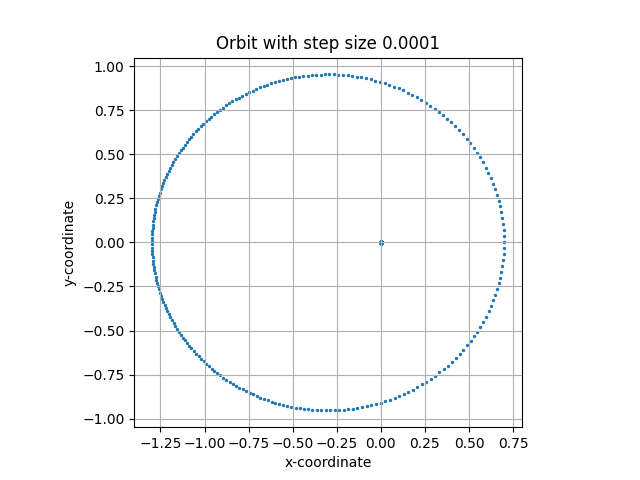
\includegraphics[width=\textwidth]{2Body/2BD0.png}
  \caption{Orbit of a two body system with leapfrog integrator and timestep of $10^{-3}$. The number of data points are less dense closer to the pericenter, which means that $m_2$ is moving faster. This follows Kepler's second law.}
  \label{fig:leapfrog_1e-3}
\end{figure}

\subsubsection{Testing for different timesteps}
Effect of smaller timesteps is tested with the leapfrog integrator with timesteps of $1$, $10^{-1}$,$10^{-2}$, $10^{-3}$,$10^{-4}$, $10^{-5}$ and $10^{-6}$.\\
\begin{figure}[H]
  \centering
  \begin{subfigure}{0.49\textwidth}
    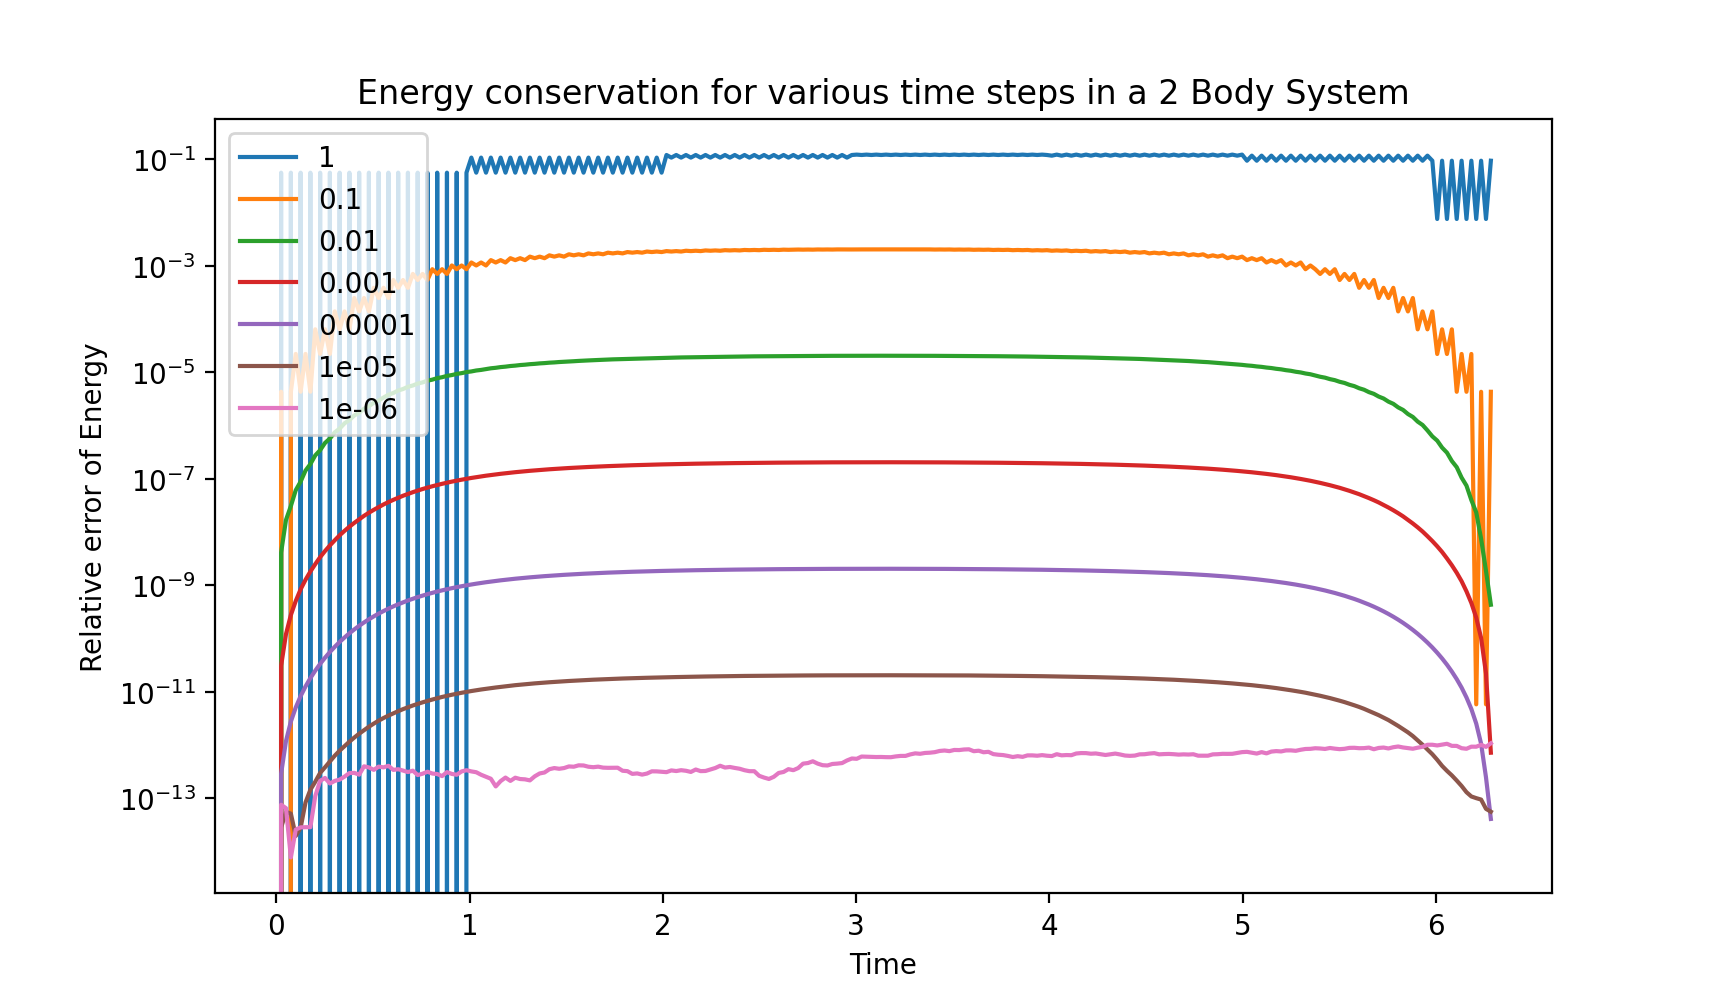
\includegraphics[height = 1.7in]{2Body/2Body_Energy_Consv_dt.png}
    \caption{Conservation of Energy at various timesteps. As we increase the timestep, the energy deviation from the initial value increases.}
    \label{fig:dt_e}  
  \end{subfigure}
  \begin{subfigure}{0.49\textwidth}
    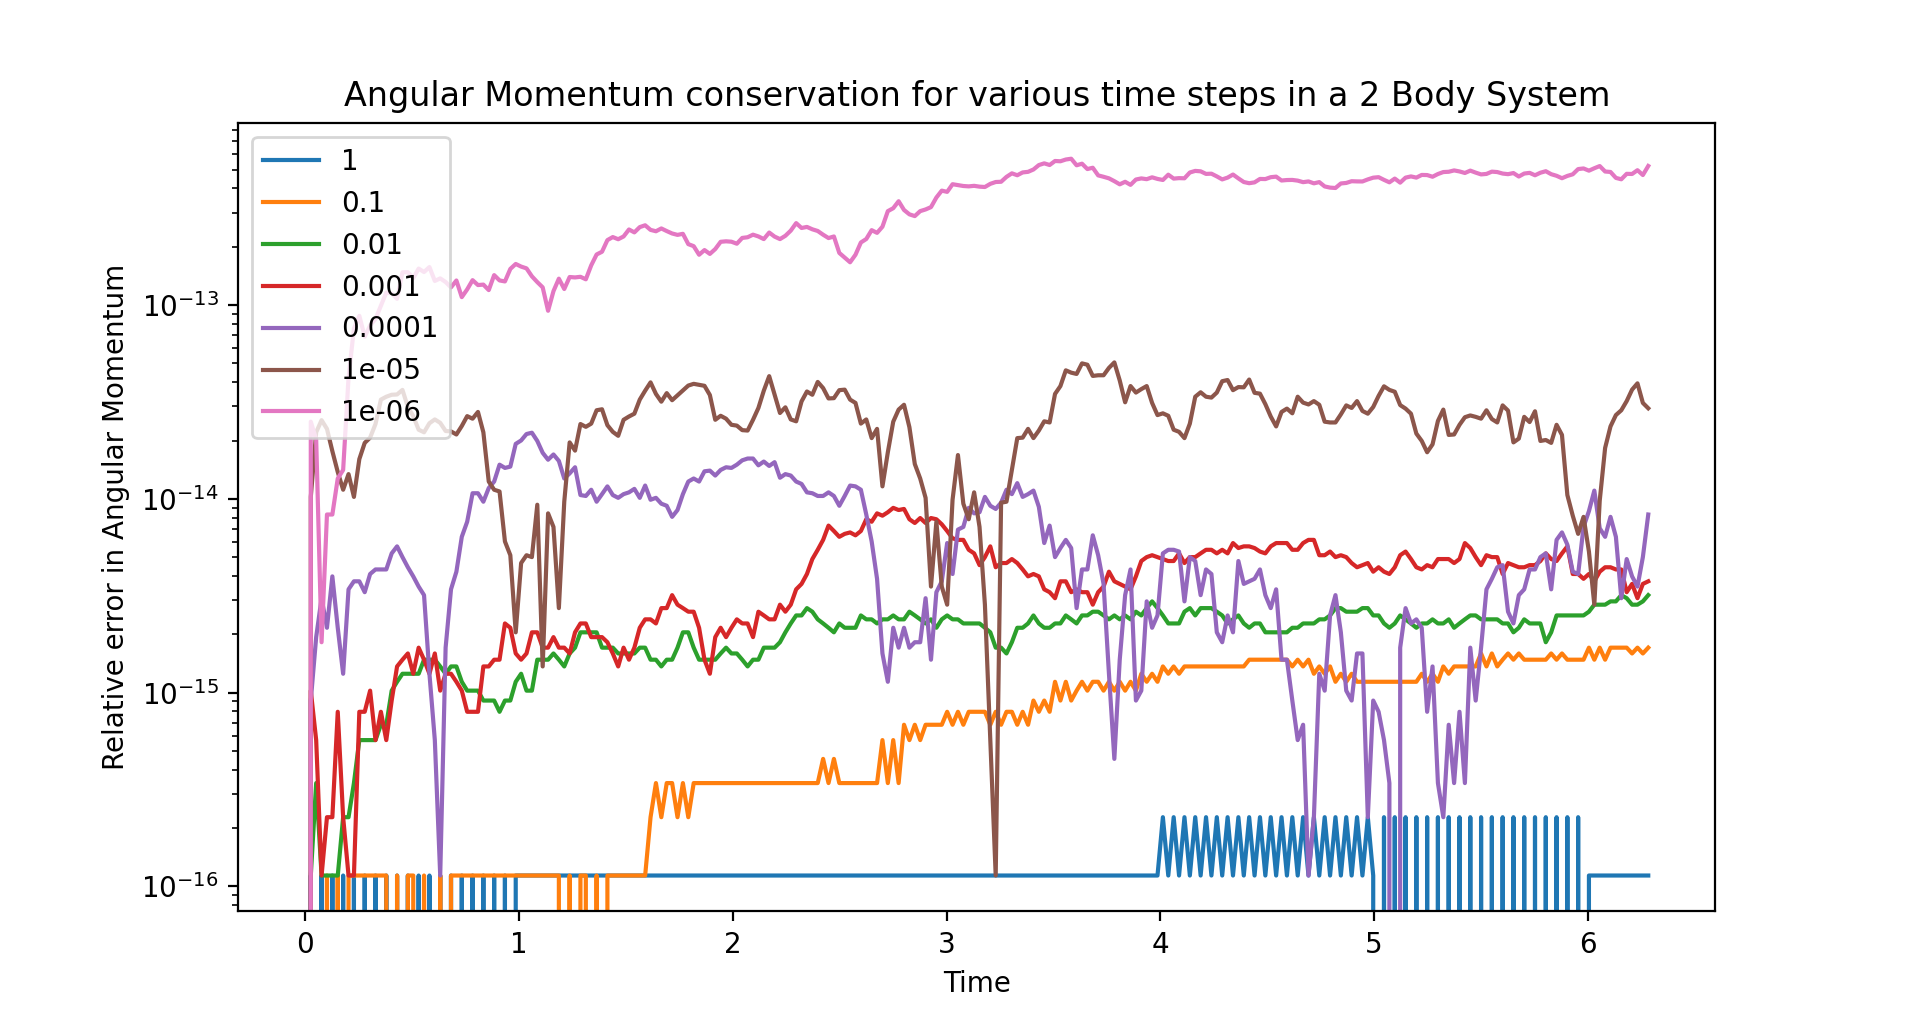
\includegraphics[height = 1.7in]{2Body/2Body_L_Consv_dt.png}
    \caption{Conservation of Angular Momentum at various timesteps. Conservation of angular momentum gets worse as we decrease the timestep.}
    \label{fig:dt_L}  
  \end{subfigure}
  \caption{Conservation of Energy and Angular Momentum at various timesteps}
\end{figure}

\begin{figure}[H]
  \centering
  \begin{subfigure}{0.49\textwidth}
    \includegraphics[height = 1.7in]{2Body/2Body_const_a_dt.png}
    \caption{Semi Major Axis at various timesteps}
    \label{fig:dt_a}  
  \end{subfigure}
  \begin{subfigure}{0.49\textwidth}
    \includegraphics[height = 1.7in]{2Body/2Body_const_ecc_dt.png}
    \caption{Eccentricity at various timesteps}
    \label{fig:dt_ecc}  
  \end{subfigure}
  \caption{Constant semi major axis and eccentricity at various timesteps}
\end{figure}
\subsubsection{Testing for different integrators}
Effect of different integrators is tested with a timestep of $10^{-3}$ using the leapfrog, IAS15, WHFast and Gragg-Bulirsch-Stoer integrators. 
The description of these Integrators is given in section \ref{integrators}.\\

% add figure
\begin{figure}[H]
  \centering
  \begin{subfigure}{0.49\textwidth}
    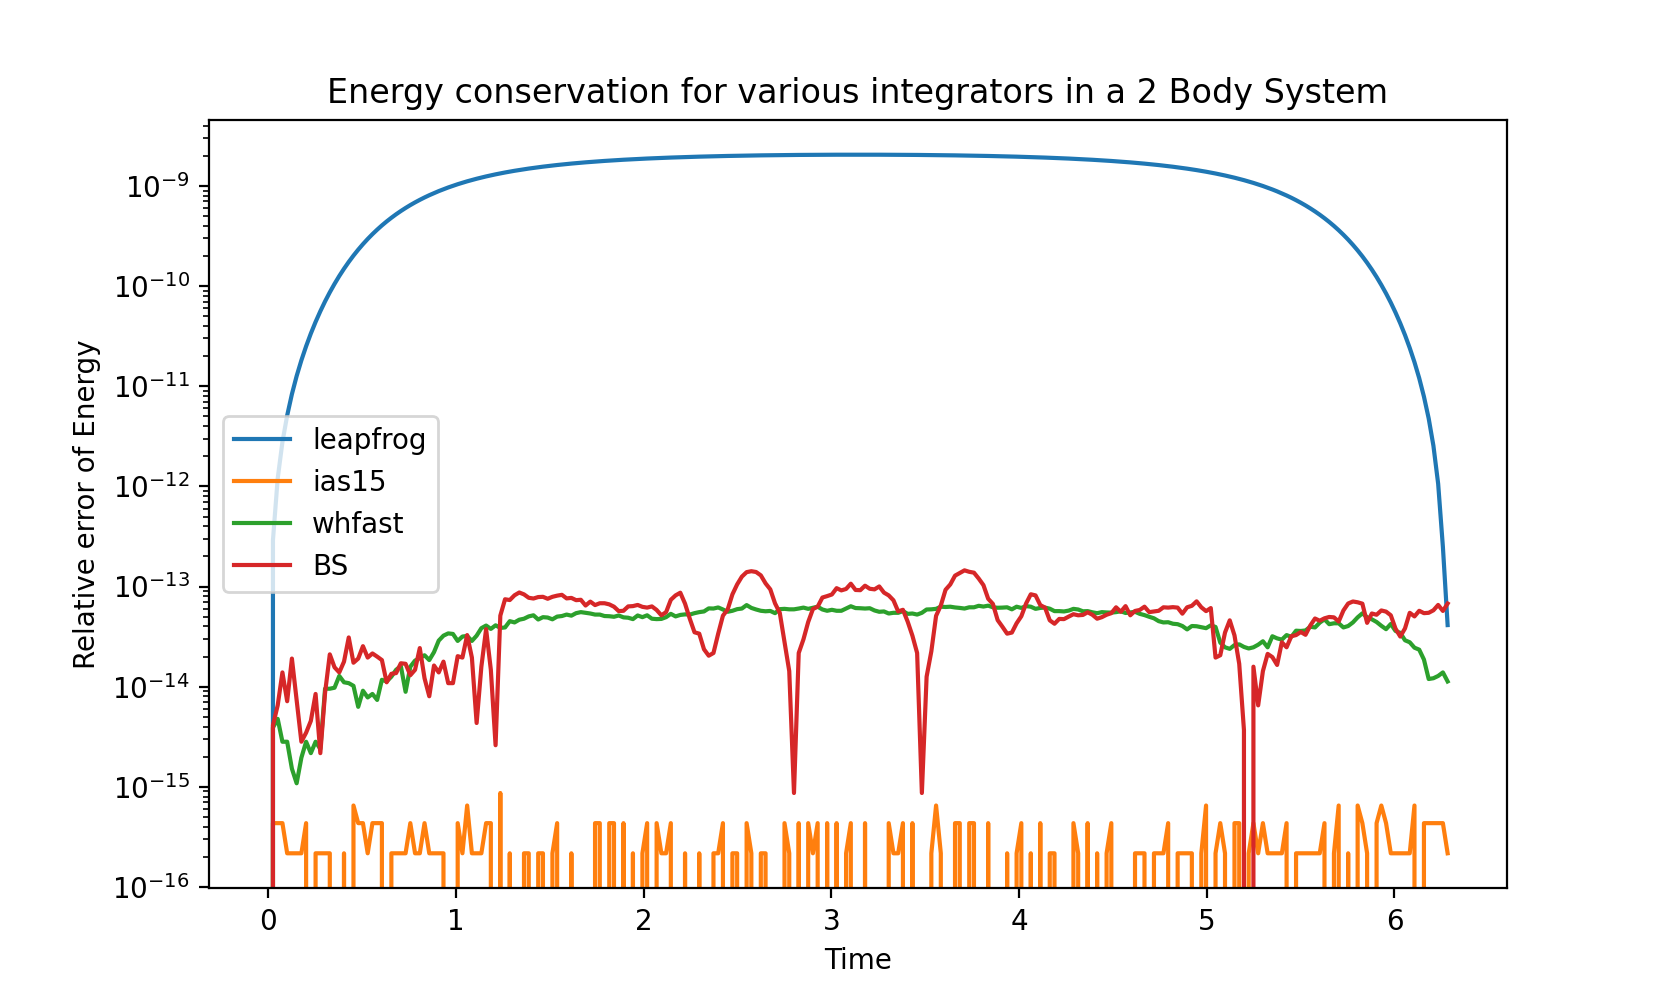
\includegraphics[height = 1.7in]{2Body/2Body_Energy_Consv_int.png}
    \caption{Conservation of Energy using different integrators}
    \label{fig:int_e}  
  \end{subfigure}
  \begin{subfigure}{0.49\textwidth}
    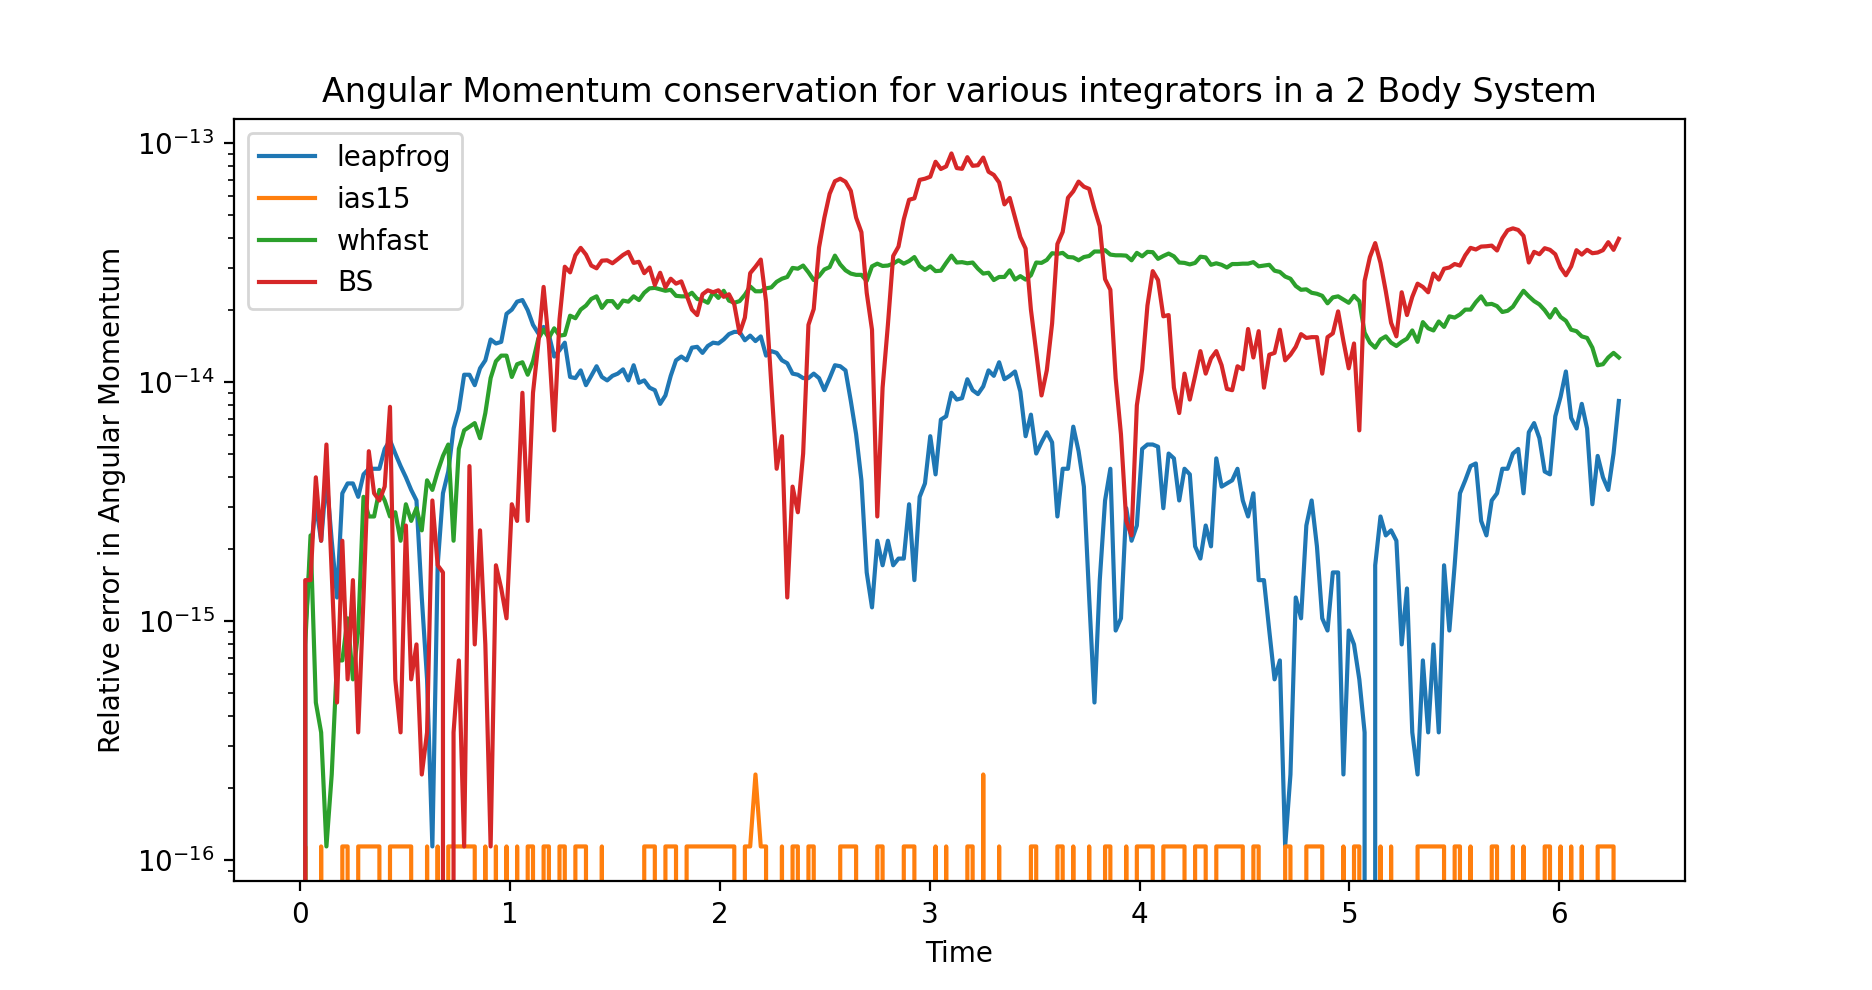
\includegraphics[height = 1.7in]{2Body/2Body_L_Consv_int.png}
    \caption{Conservation of Angular Momentum using different integrators}
    \label{fig:int_L}  
  \end{subfigure}
  \caption{Conservation of Energy and Angular Momentum using different integrators}
  \label{fig:int:4}
\end{figure}

\begin{figure}[H]
  \centering
  \begin{subfigure}{0.49\textwidth}
    \includegraphics[height = 1.7in]{2Body/2Body_const_a_int.png}
    \caption{Semi Major Axis using different integrators}
    \label{fig:int_a}  
  \end{subfigure}
  \begin{subfigure}{0.49\textwidth}
    \includegraphics[height = 1.7in]{2Body/2Body_const_ecc_int.png}
    \caption{Eccentricity using different integrators} 
    \label{fig:int_ecc}  
  \end{subfigure}
  \caption{Constant semi major axis and eccentricity using different integrators}
  \label{fig:int:5}
\end{figure}

From figure \ref{fig:int:4} and figure \ref{fig:int:5} we can see that the IAS 15 integrator is significantly more accurate than the other integrators. WHFast and Gragg-Bulirsch-Stoer integrators have similar accuracy while
 the leapfrog integrator is the least accurate.
\subsection{Three Body Problem and Stability of the Planet System}
Here we will simulate a coplanar 3 body system with a large central mass $(m_1)$ and two smaller masses $(m_2, m_3)$ in circular orbits. The two small objects will start opposite to each other (at a 
phase difference of $\pi$). We vary the distance  between $m_2$ and $m_3$ to study the stability of the system.\\
The eccentricity and the semi major axis of the bodies will vary due to gravitational perturbations from the other bodies. For bodies that are closer, the gravitational perturbations will be larger which will result in
stronger changes for the eccentricities and semi major axis. For initially circular orbits, Gladman\cite{Gladman} defined a criterion for the stability of the system:
\begin{equation}
  \Delta_c \simeq 2.40(\mu_2+\mu_3)^{1/3}
\end{equation}
Where $\mu$ is the mass ratio with respect to $m_1$. %CHECK THIS
At distances greater than $\Delta_c$, the system is considered to be stable. When the system is unstable, there is a possibility of close encounters between $m_1$ and $m_2$. A `close encounter' is when the distance between 
the two bodies is less than the Hill radius of the larger of the two bodies. Here, the Hill radius is given by:
\begin{equation}
  R_{in} = a^3\sqrt{\mu/3}
\end{equation}
If there are no close encounters between the bodies at all times, the system is `Hill stable' or simply stable.\\
We simulate the 3 body problem using REBOUND by following a similar procedure to the 2 body problem. Using the IAS15 integrator to achieve high accuracy we simulate the system for 1000 orbits for different separations 
between the two smaller bodies. REBOUND can automatically detect close encounters between the bodies and handle them accordingly (halting the simulation, merging the bodies, hard sphere collision or a user defined function). 
For our purposes we will only count the number of close encounters.\\
\subsubsection{Equal Mass Planets}
We  simulate the system with $m_1=1$, $m_2=m_3=10^-5$,$a_1=1$,$a_2=1+\Delta$ where $\Delta$ is the separation between the two smaller bodies. The eccentricities of both bodies is initially 0. We create different simulations for
$\Delta = 0.1, 0.5, 1, 1.5$ and $10$ times the value of $\Delta_c$ for this system.
As expected, for $\Delta\geq\Delta_c$ the orbits are stable. For $\Delta=1\Delta_c$ and $\Delta=1.5\Delta_c$ the planets are in resonances.
\begin{figure}[H]
  \begin{subfigure}{0.49\textwidth}
    \centering
    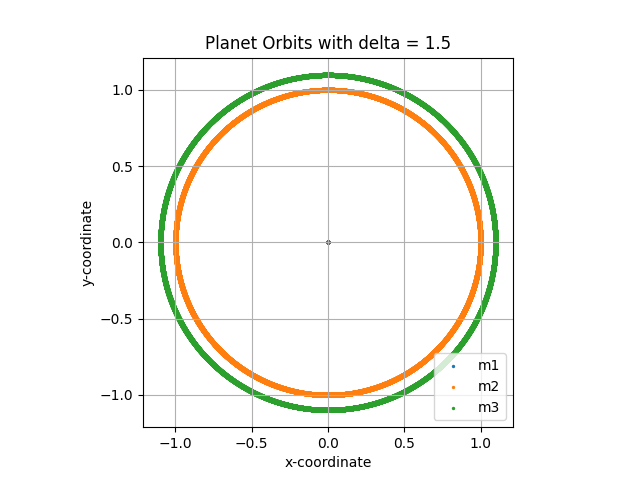
\includegraphics[height = 2.3in]{3Body/3BD_orbit_delta1.5.png}
    \caption{Orbit of a 3 body system with $\Delta = 1.5\Delta_c$. The system is stable and the planets are in a 3:2 resonance}
    \label{fig:3Body_1.5}
  \end{subfigure}
  \begin{subfigure}{0.49\textwidth}
    \centering
    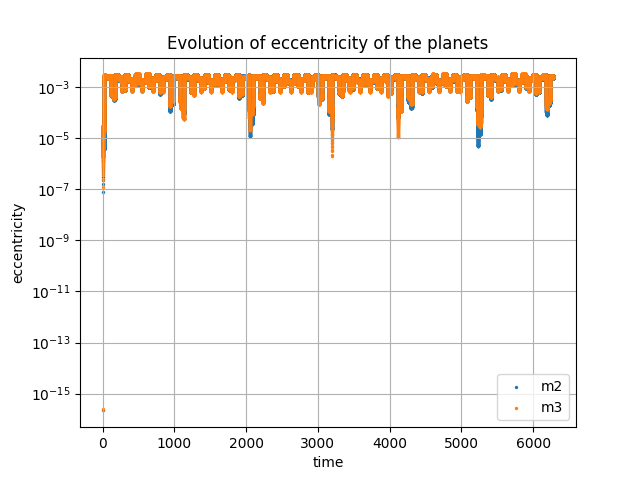
\includegraphics[height = 2.3in]{3Body/3BD_ecc_delta1.5.png}
    \caption{Eccentricity of the planets with $\Delta = 1.5\Delta_c$. It is same for both planets throughout its evolution}
    \label{fig:3Body_1.5_ecc}
  \end{subfigure}
  
  \begin{subfigure}{0.49\textwidth}
    \centering
    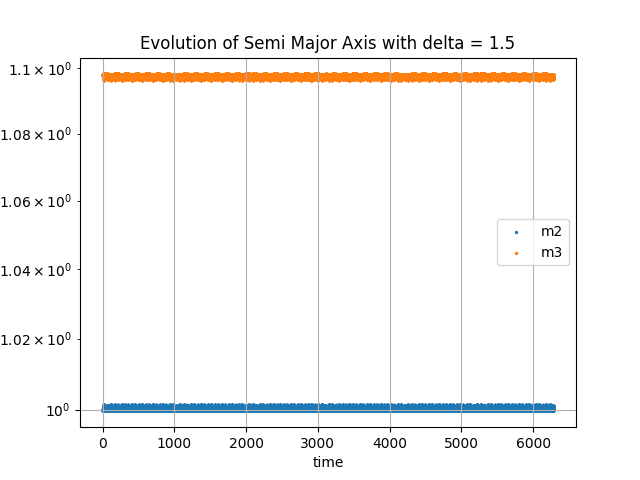
\includegraphics[height = 2.1in]{3Body/3BD_a_delta1.5.png}
    \caption{Semi Major Axis of the planets with $\Delta = 1.5\Delta_c$. It is basically constant}
    \label{fig:3Body_1.5_a}
  \end{subfigure}
  \caption{Properties of a 3 body system with $\Delta = 1.5\Delta_c$}
\end{figure}

For $\Delta=10\Delta_c$, we observe the effect of tidal forces and observe the eccentricity of the closer planet increase
\begin{figure}[H]
  % \begin{subfigure}{0.49\textwidth}
  \centering
  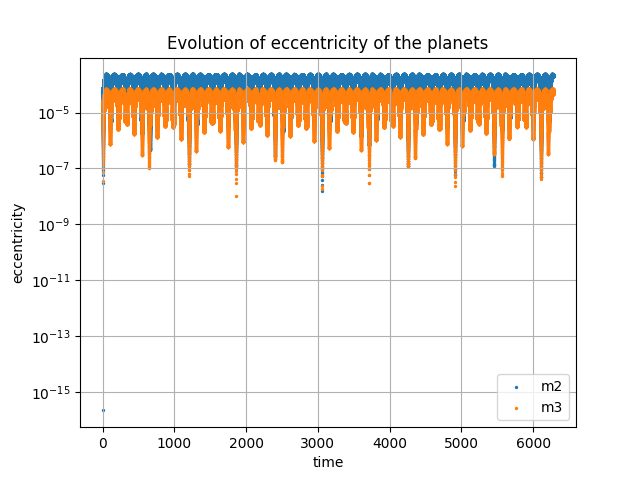
\includegraphics[height = 2.7in]{3Body/3BD_ecc_delta10.png}
  \caption{Eccentricity of the planets with $\Delta = 10\Delta_c$. An increase in eccentricity for the planet closer to the star($m_2$) is observed}
  \label{fig:3Body_10}
  % \end{subfigure}
\end{figure}

For $\Delta=0.1\Delta_c$ we observe that the planets periodically exchange their orbits. Even though this is less than $\Delta_c$, there are no close encounters
detected by REBOUND.
\begin{figure}[H]
  \centering
  \begin{subfigure}{0.49\textwidth}
    \centering
    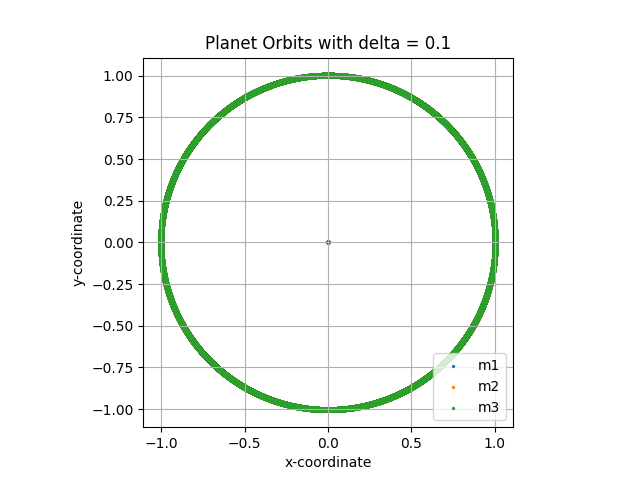
\includegraphics[height = 2.4in]{3Body/3BD_orbit_delta0.1.png}
    \caption{Orbit of a 3 body system with $\Delta = 0.1\Delta_c$. In this plot both of the planet orbits are on top of each other}
    \label{fig:3Body_0.1}
  \end{subfigure}
  \begin{subfigure}{0.49\textwidth}
    \centering
    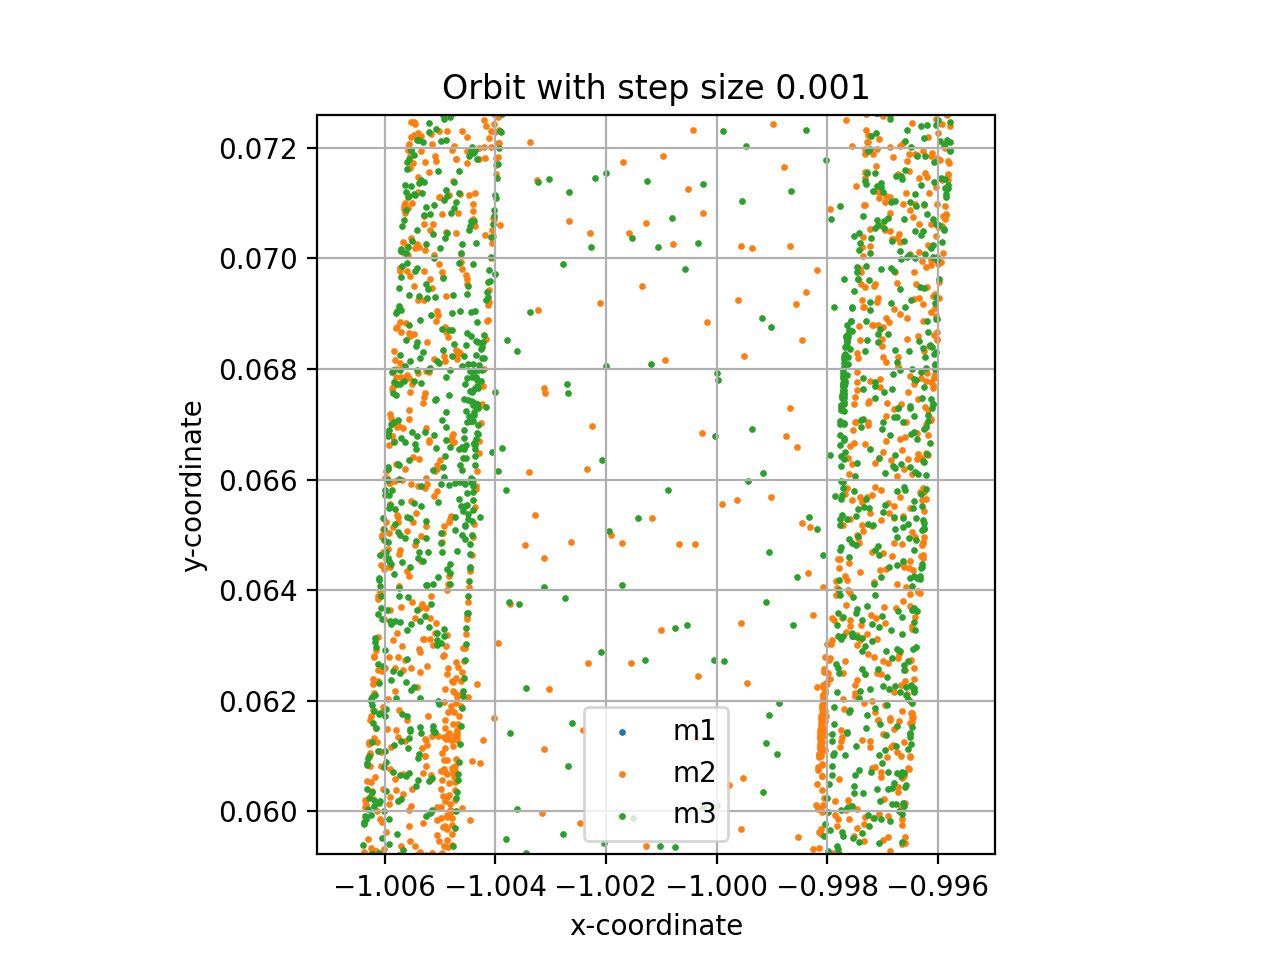
\includegraphics[height = 2.4in]{3Body/3BD_orbit_delta0.1_Close.png}
    \caption{A closer view of the orbit. The exchange of orbits is clearly observed here}
    \label{fig:3Body_0.1_close}
  \end{subfigure}

  \begin{subfigure}{0.49\textwidth}
    \centering
    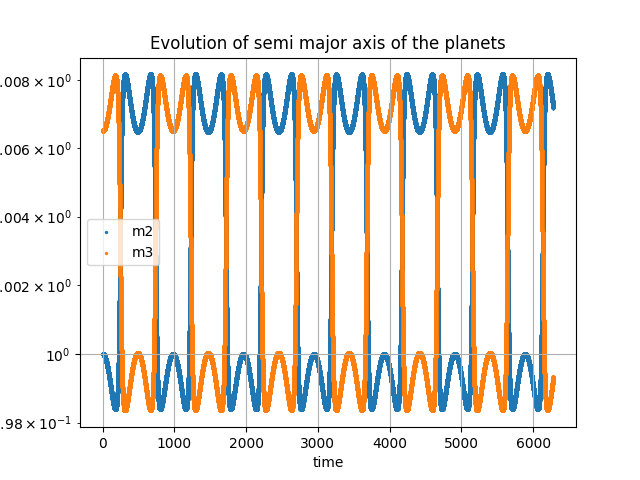
\includegraphics[height = 2.4in]{3Body/3BD_a_delta0.1.png}
    \caption{Change in semi major axis of the planets with $\Delta = 0.1\Delta_c$. The orbit exchange is clearly observed here}
    \label{fig:3Body_0.1_close}
  \end{subfigure}
  \caption{Orbit of a 3 body system with $\Delta = 0.1\Delta_c$}
\end{figure}

For $\Delta=0.5\Delta_c$ the system is unstable and REBOUND detects several collisions here (in our case$ \sim $ 11,000 collisions but this can vary depending on the type of integrator or time step).

\begin{figure}[H]
  \centering
  % \begin{subfigure}{0.4\textwidth}
  %   \centering
  %   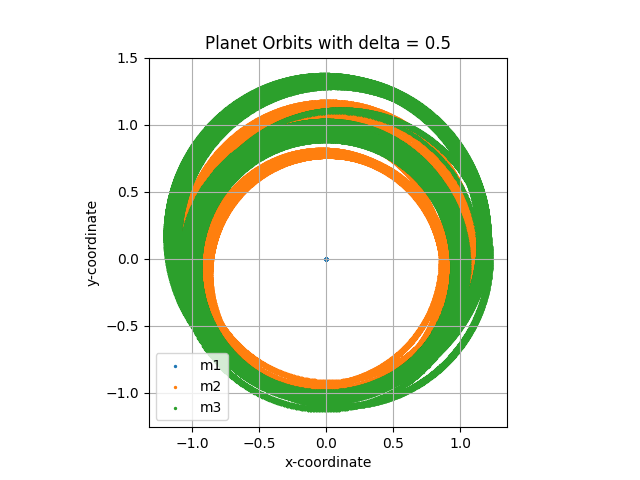
\includegraphics[height = 2.4in]{3Body/3BD_orbit_delta0.5.png}
  %   \caption{Orbit of a 3 body system with $\Delta = 0.5\Delta_c$}
  %   \label{fig:3Body_0.5}
  % \end{subfigure}
  \begin{subfigure}{0.4\textwidth}
    \centering
    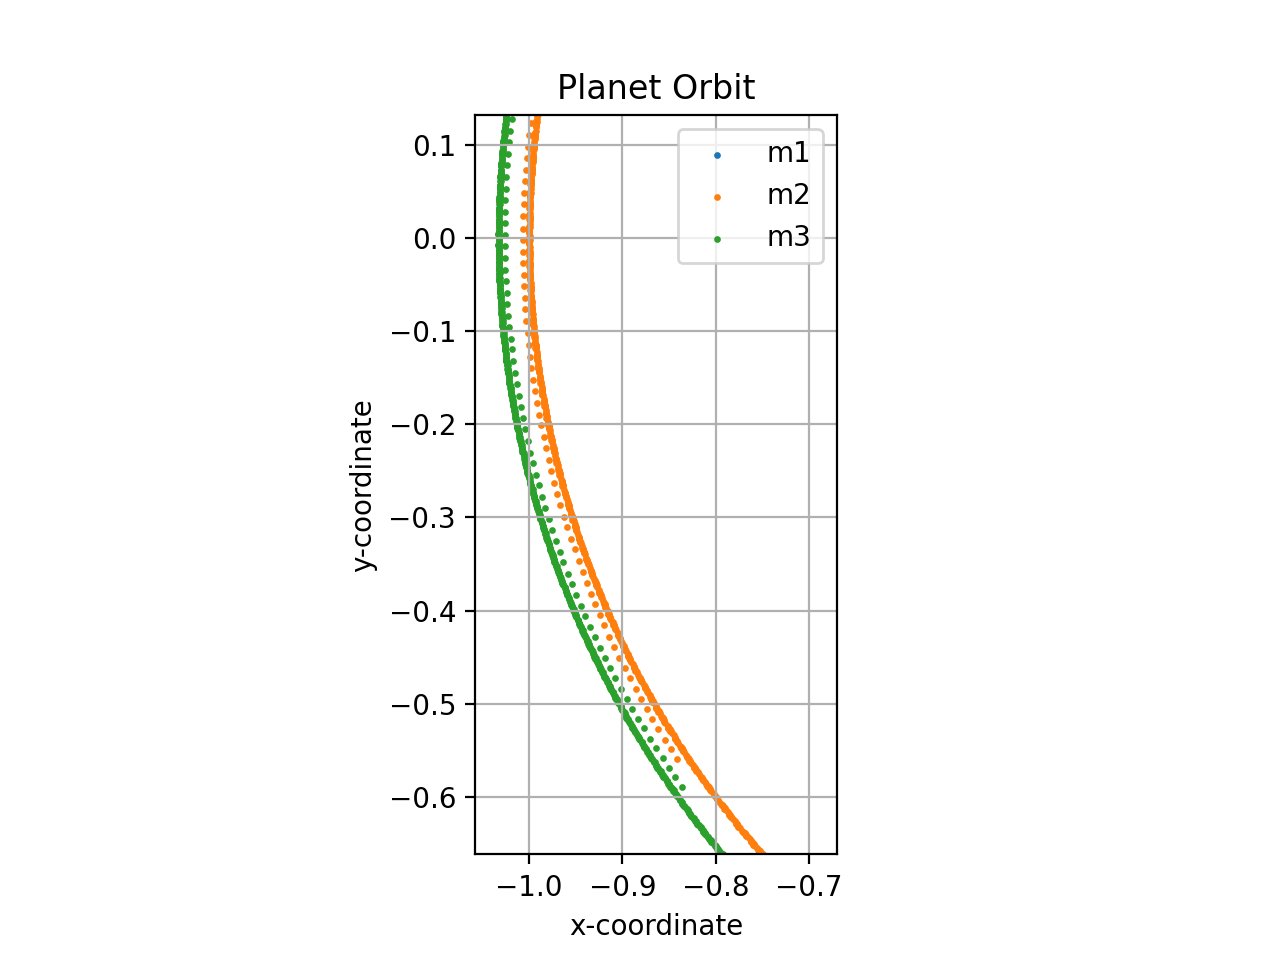
\includegraphics[height = 2.4in]{3Body/3BD_orbit_delta0.5_till_collision.png}
    \caption{Close view of the orbit plotted till the first collision is detected}
    \label{fig:3Body_0.5_short}
  \end{subfigure}
  \begin{subfigure}{0.4\textwidth}
    \centering
    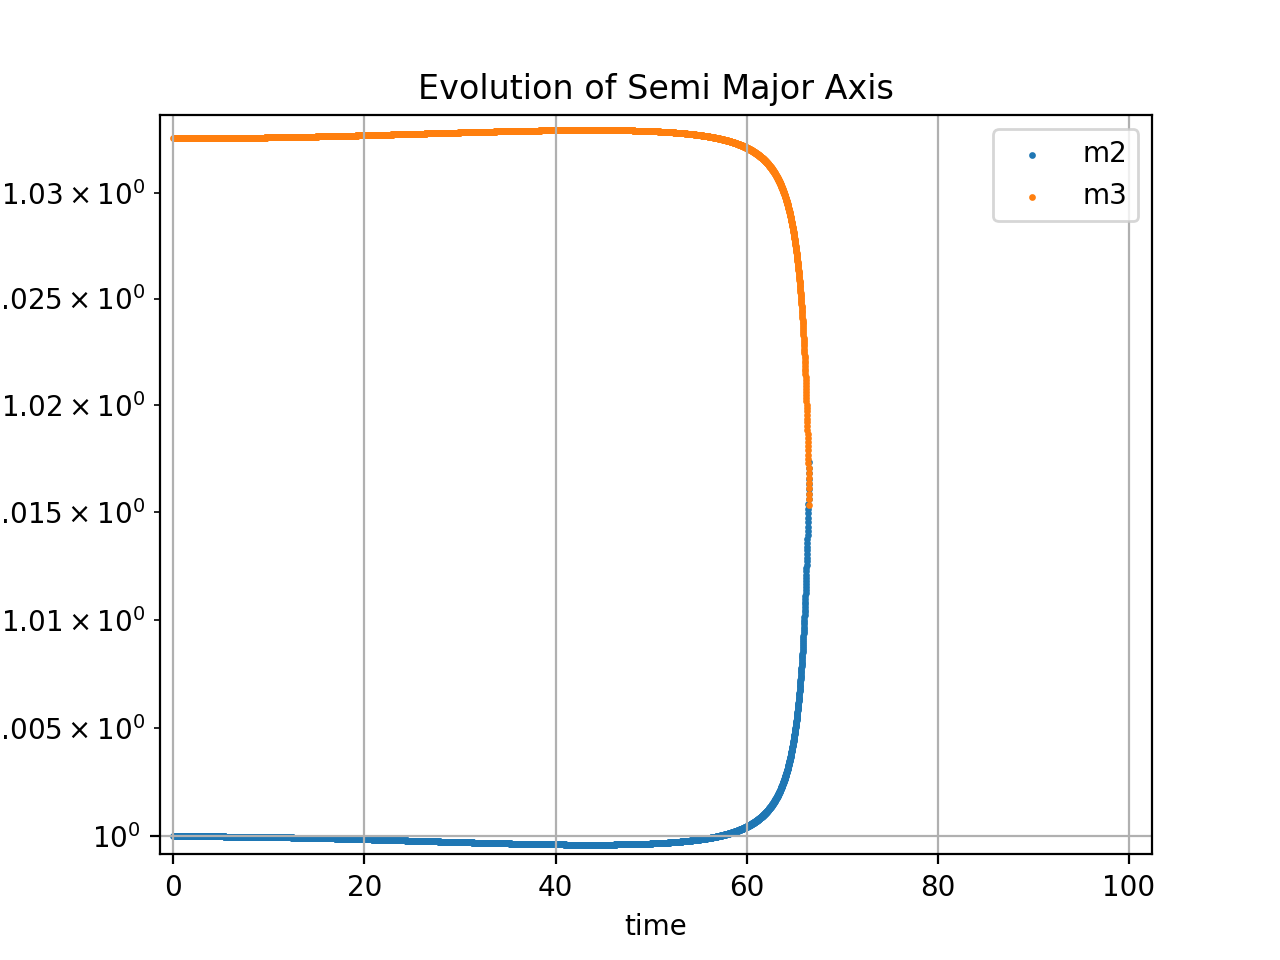
\includegraphics[height = 2.4in]{3Body/3BD_a_delta0.5_till_collision.png}
    \caption{Change in semi major axis of the planets with $\Delta = 0.5\Delta_c$ till first collision}
    \label{fig:3Body_0.5_a}
  \end{subfigure}

  \begin{subfigure}{0.4\textwidth}
    \centering
    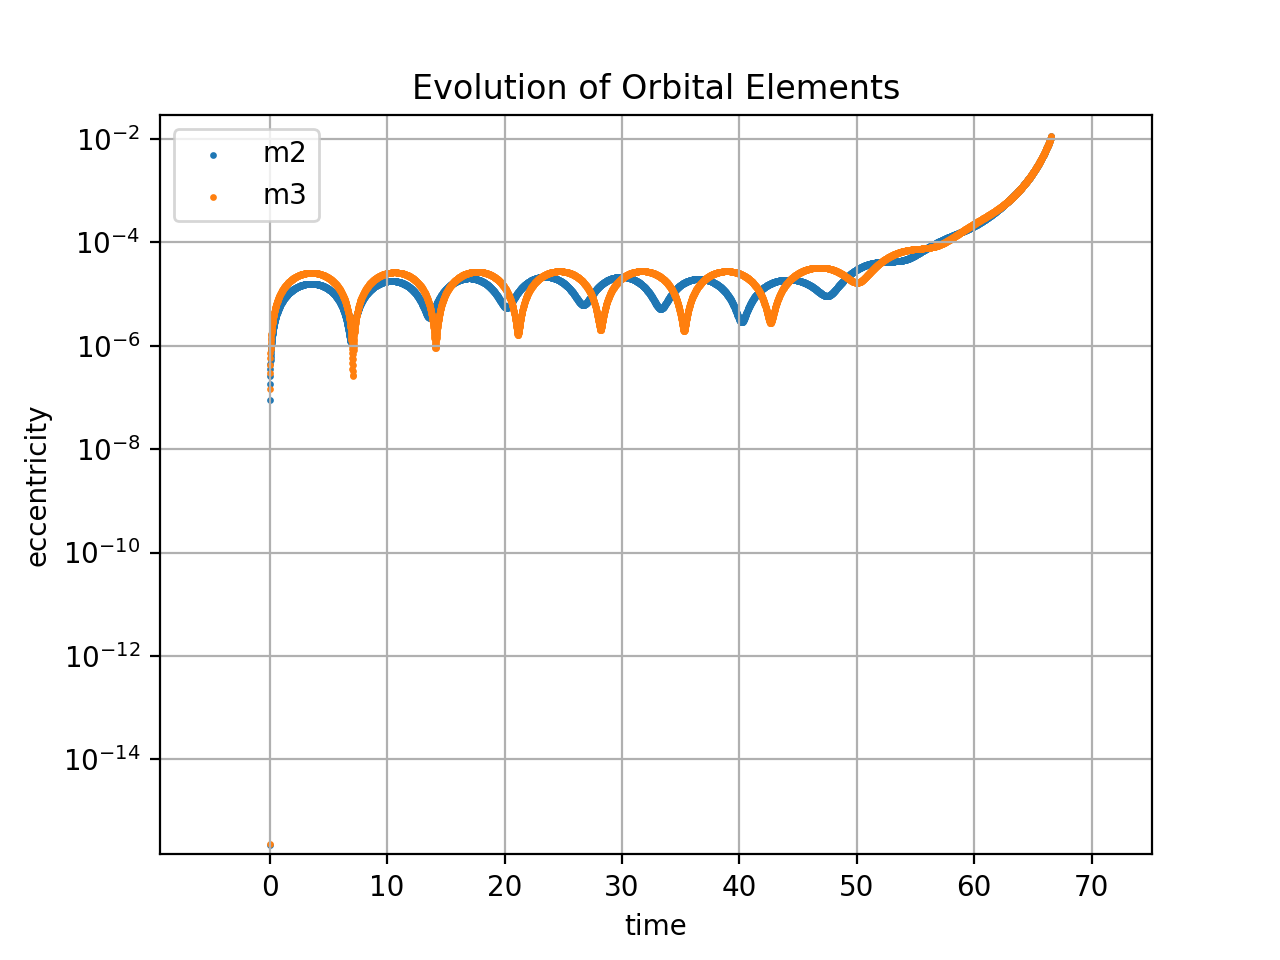
\includegraphics[height = 2.4in]{3Body/3BD_ecc_delta0.5_till_collision.png}
    \caption{Change in eccentricity of the planets with $\Delta = 0.5\Delta_c$ till first collision}
    \label{fig:3Body_0.5_ecc}
  \end{subfigure}
  \caption{Properties of a 3 body system with $\Delta = 0.5\Delta_c$}
\end{figure}
\subsubsection{Unequal Mass Planets}
The above exercise was repeated by changing one of the masses $m_3= 10^{-7}$. \\
For $\Delta=0.1\Delta_c$ the orbit exchange is still observed, but now the smaller planet $m_3$ has a larger variation in semi major axis as compared to $m_2$.
\begin{figure}[H]
  \centering
  \begin{subfigure}{0.49\textwidth}
    \centering
    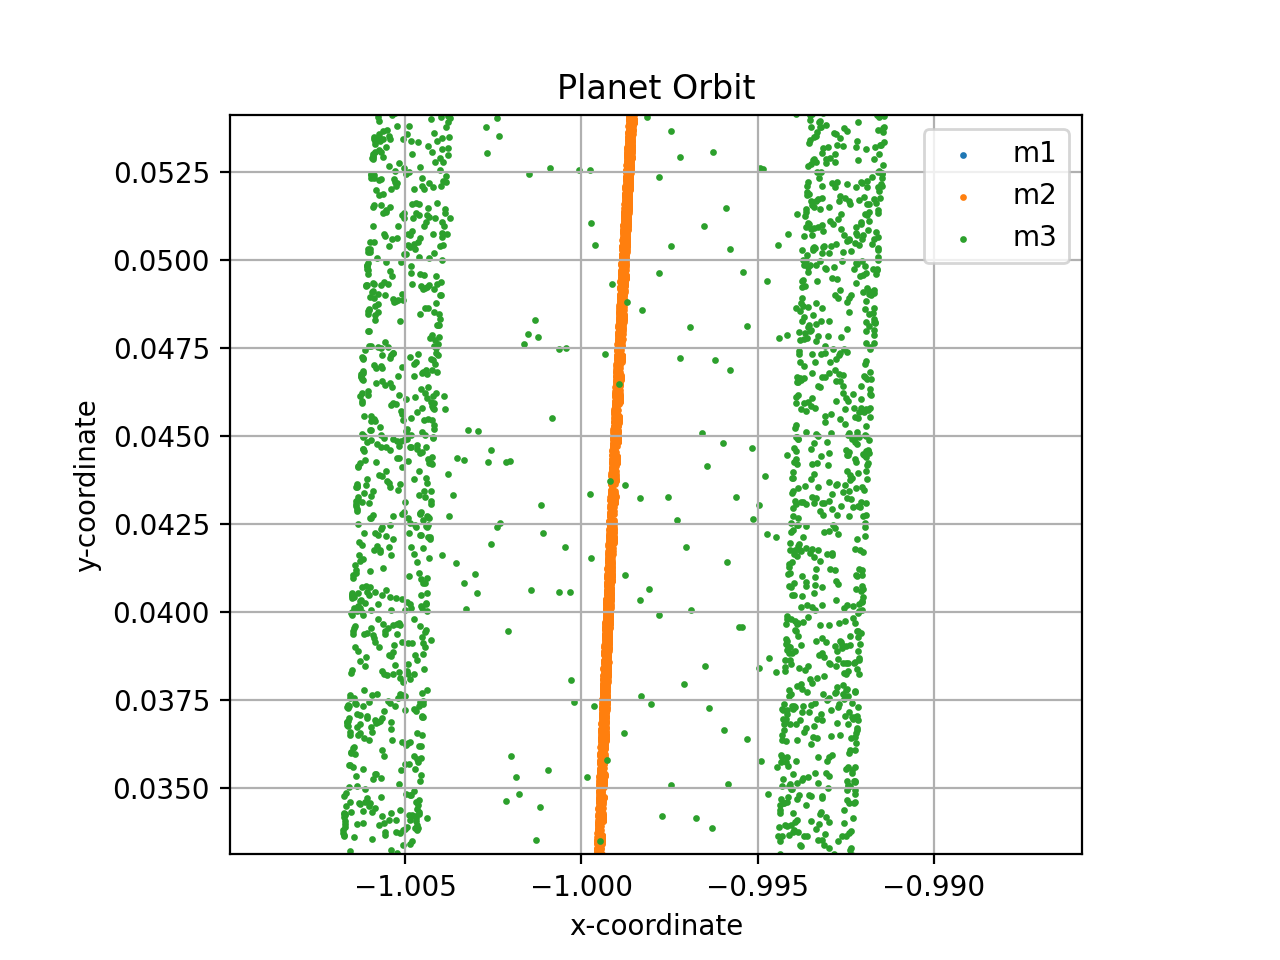
\includegraphics[height = 2.4in]{3Body/3BD_orbit_delta0.1_Close_2.png}
    \caption{A closer view of the orbit}
    \label{fig:3Body_0.1_close_ueq}
  \end{subfigure}

  \begin{subfigure}{0.49\textwidth}
    \centering
    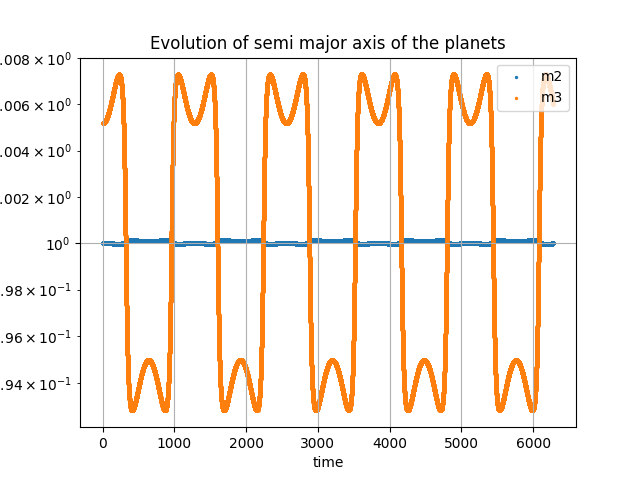
\includegraphics[height = 2.4in]{3Body/3BD_a_delta_20.1.png}
    \caption{Change in semi major axis of the planets with $\Delta = 0.1\Delta_c$ for planets of different masses}
    \label{fig:3Body_0.1_close_ueq_a}
  \end{subfigure}
  \caption{Orbit of a 3 body system with $\Delta = 0.1\Delta_c$. In both graphs we observe that the smaller planet has a larger variation in semi major axis}
\end{figure}
Now, REBOUND detects collisions for both $\Delta=0.5\Delta_c$ and $\Delta=1\Delta_c$.\\
\begin{figure}[H]
  \centering
  \begin{subfigure}{0.4\textwidth}
    \centering
    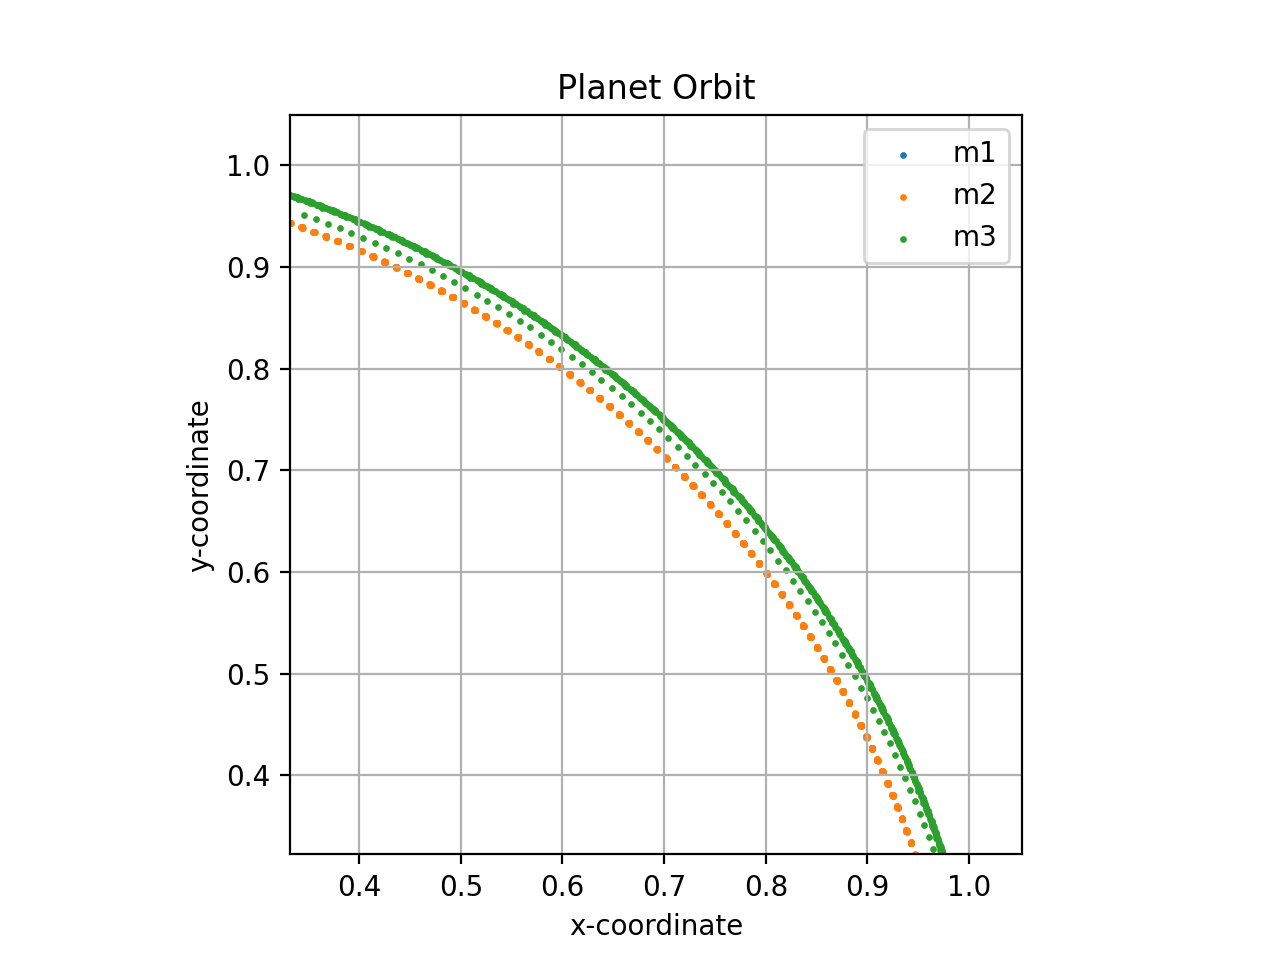
\includegraphics[height = 2.4in]{3Body/3BD_orbit_delta_2_0.5_collide.png}
    \caption{Close view of the orbit plotted till the first collision is detected}
    % \label{fig:3Body_0.5_short}
  \end{subfigure}
  \begin{subfigure}{0.4\textwidth}
    \centering
    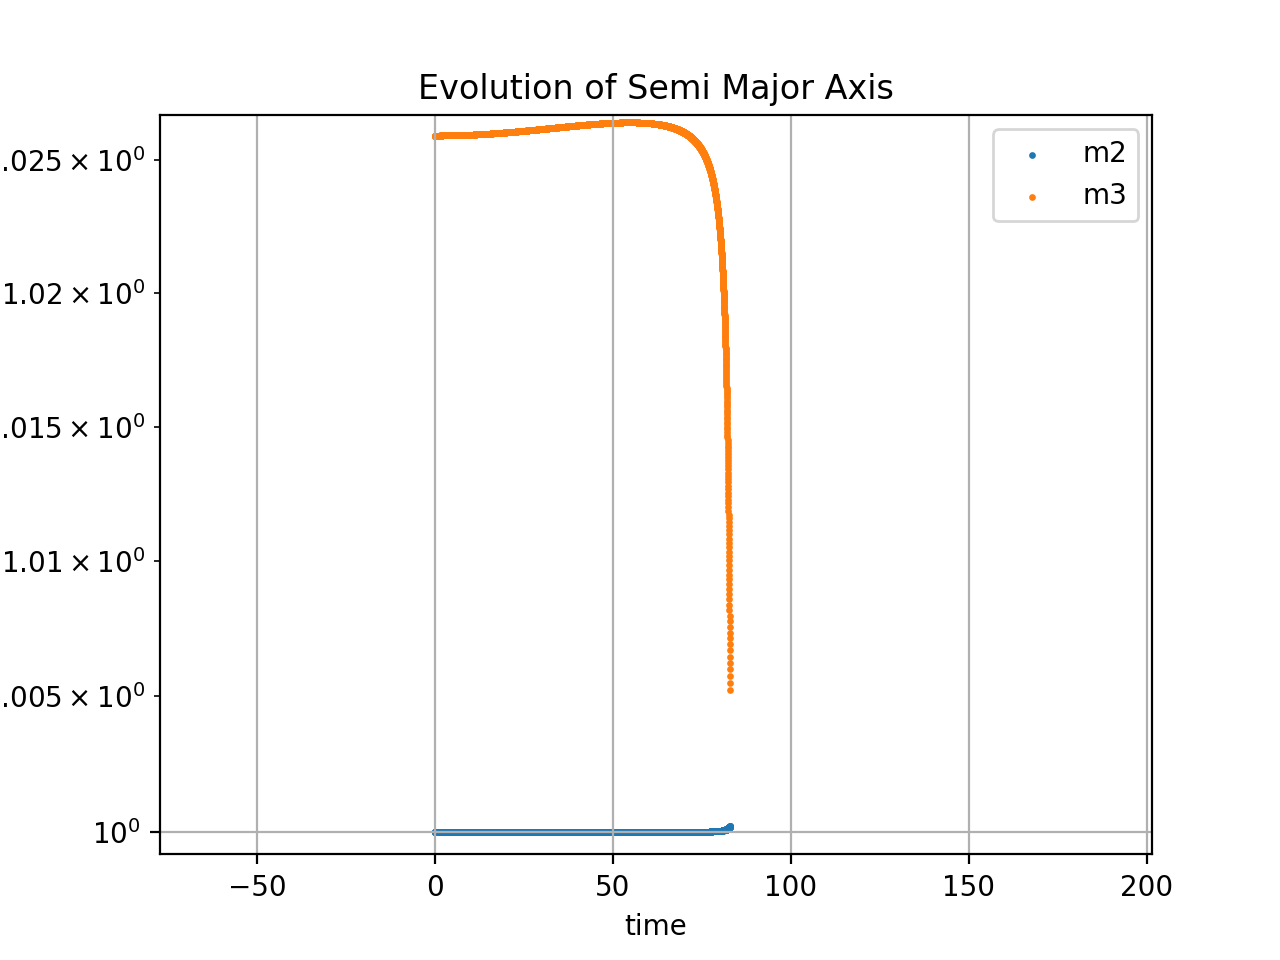
\includegraphics[height = 2.4in]{3Body/3BD_a_delta_2_0.5_collide.png}
    \caption{Change in semi major axis of the planets with $\Delta = 0.5\Delta_c$ till first collision. The smaller planet travels a larger distance before collision}
    % \label{fig:3Body_0.5_a}
  \end{subfigure}

  \begin{subfigure}{0.4\textwidth}
    \centering
    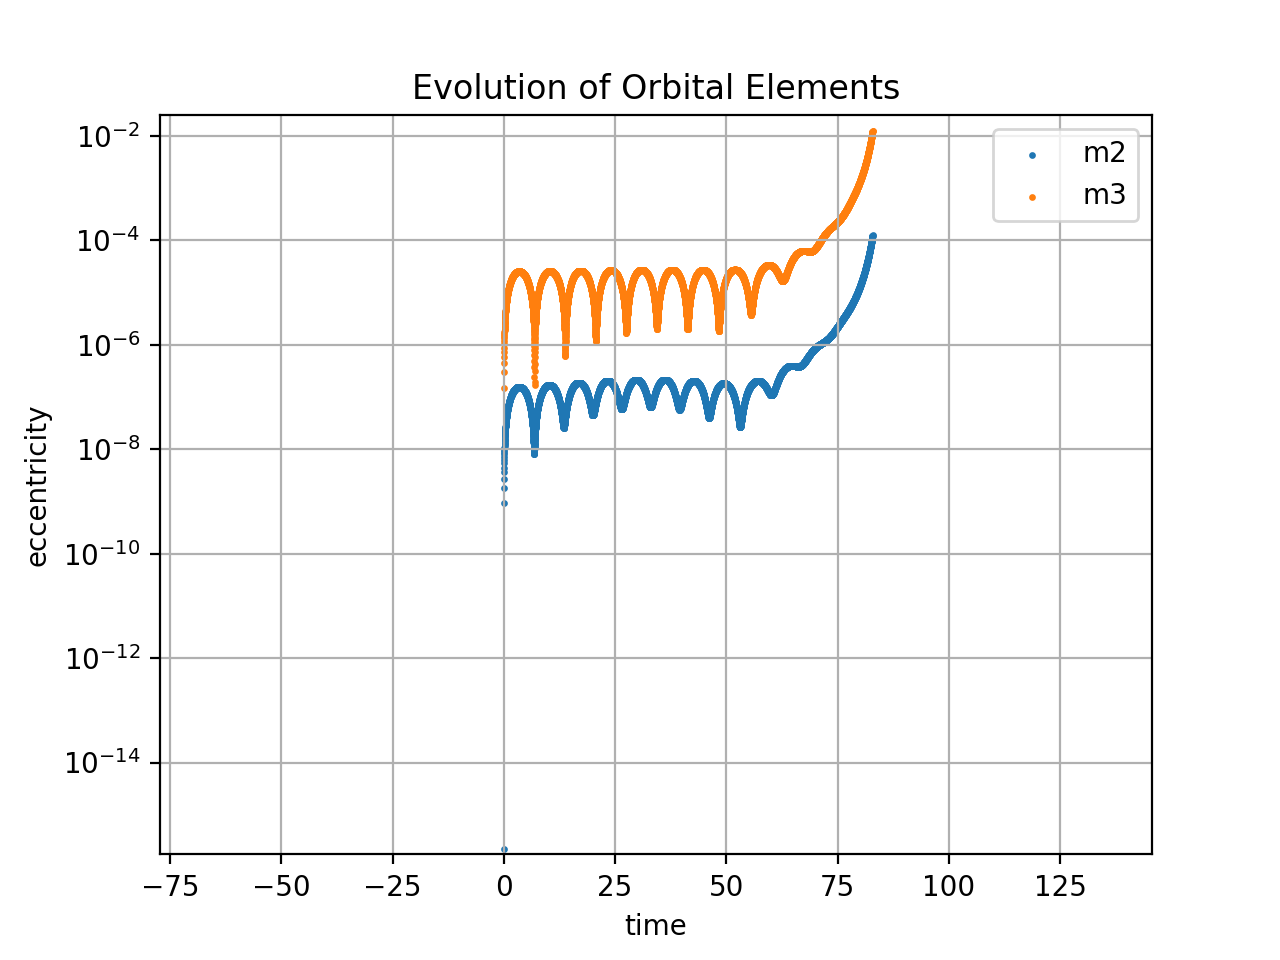
\includegraphics[height = 2.4in]{3Body/3BD_ecc_delta_2_0.5_collide.png}
    \caption{Change in eccentricity of the planets with $\Delta = 0.5\Delta_c$ till first collision}
    % \label{fig:3Body_0.5_ecc}
  \end{subfigure}
  \caption{Properties of a 3 body system with $\Delta = 0.5\Delta_c$ and with masses $m_2=10^{-5}$ and $m_3=10^{-7}$}
\end{figure}
Systems with higher $\Delta_c$ are still stable

\begin{figure}
  \centering
  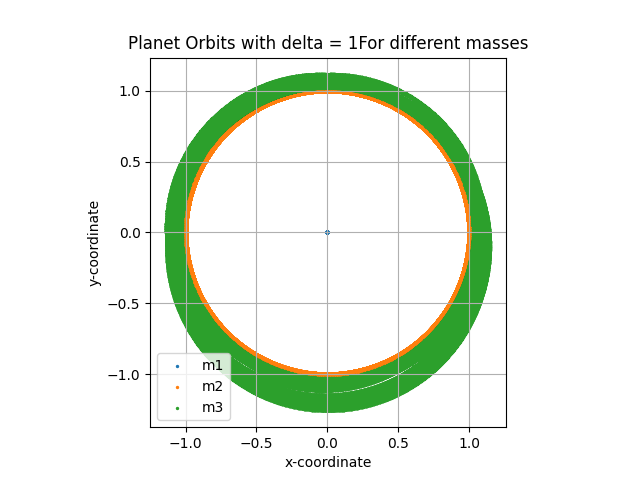
\includegraphics[height = 2.4in]{3Body/3BD_orbit_delta_21.png}
  \caption{Orbit of a 3 body system with $\Delta = 1\Delta_c$ with unequal masses. The system is unstable}
  % \label{fig:3Body_0.5_ecc}
\end{figure}

Looking at the evolution of eccentricities with different seperations, we observe that $m_2$ has a lower eccentricity than $m_3$ in all cases
\begin{figure}[H]
  \centering
  \begin{subfigure}{0.49\textwidth}
    \centering
    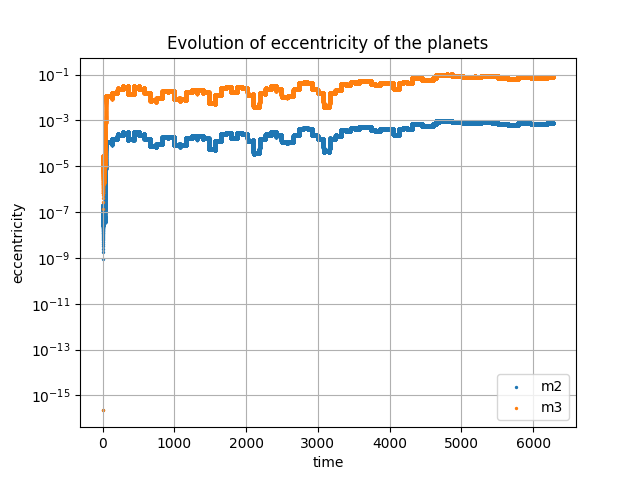
\includegraphics[height = 2.4in]{3Body/3BD_ecc_delta_21.png}
    \caption{Change in eccentricity of the planets with $\Delta = 1\Delta_c$}
    % \label{fig:3Body_0.5_short} 
  \end{subfigure}
  \begin{subfigure}{0.49\textwidth}
    \centering
    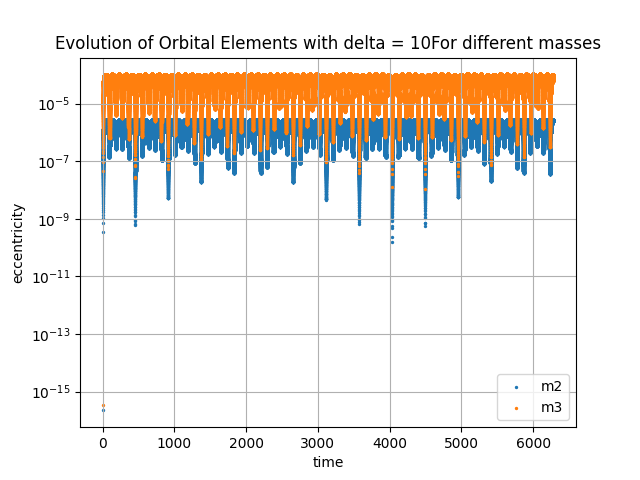
\includegraphics[height = 2.4in]{3Body/3BD_ecc_delta_210.png}
    \caption{Change in eccentricity of the planets with $\Delta = 10\Delta_c$}
    % \label{fig:3Body_0.5_a}
  \end{subfigure}
  \caption{Change in eccentricity of the planets with different separations and unequal masses}
\end{figure}
\subsection{Jupiter and Kirkwood Gaps}

In this part of the lab work we must observe Kirkwood gaps - gaps in the asteroid belt - by simulationg and observing the evolution of Sun-Jupiter-Mars system with 10000 test particles. 
Using REBOUND we can simulate these objects and get semi-major axis and eccentricity of all bodies up to 1 million years of evolution. Additionally, we check the change of distibution at every 100000 years.

Kirkwood gaps are caused by the resonant interaction between the asteroids and Jupiter \cite{asteroids}. The resonant interaction leads to the instability of the orbits of the asteroids.
Moreover, the instabilities cause the increase of eccentricity of the asteroids, and the asteroids with higher eccentricity are more likely to collide with inner planets.
The main Kirkwood gaps are at 2.50, 2.82, 2.95, 3.27 AU corresponding to the resonant periods of 3:1, 5:2, 7:3, 2:1 respectively.

The observed distribution of asteroids in the asteroid belt are shown in Fig. \cite{fig:real_kirkwood} below:

\begin{figure}[H]
  \centering
  \begin{subfigure}{0.49\textwidth}
    \centering
    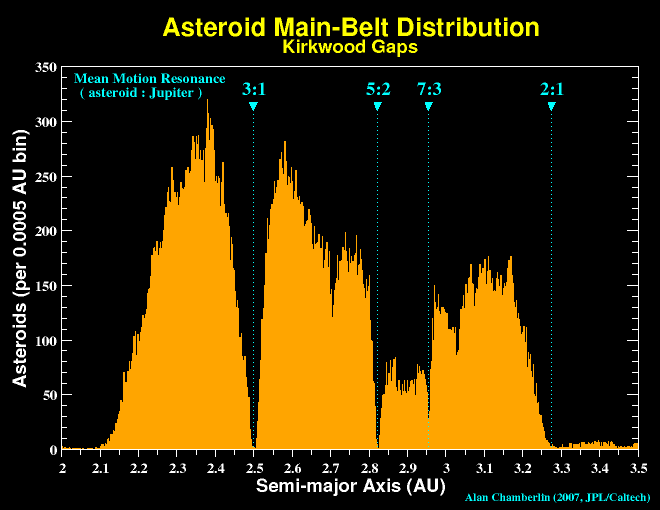
\includegraphics[width=\linewidth]{kirkwood/kirkwood.png}
  \end{subfigure}
  \begin{subfigure}{0.49\textwidth}
    \centering
    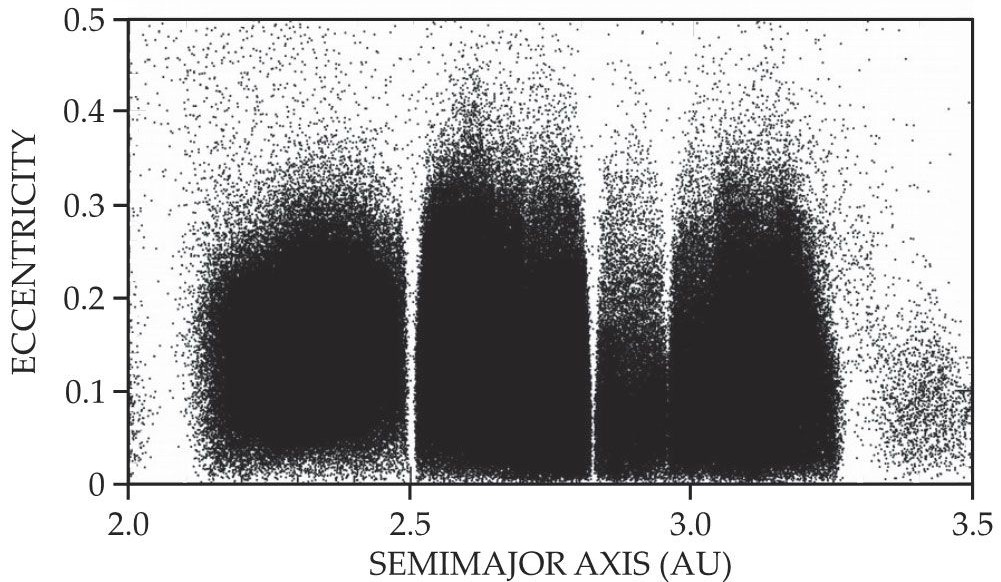
\includegraphics[width=\linewidth]{kirkwood/eccentricity_semimajor.jpeg}
  \end{subfigure}
  \caption{Number distribution of asteroids and eccentricity vs semi-major axis distributions from observed data.}
  \label{fig:real_kirkwood}
\end{figure}

Our task is to simulate these results using REBOUND.

First, Sun, Jupiter and Mars are added with their corresponding masses, semi-major axes and eccentricities. 
Next, we add 10000 test particles in a range of 2 to 4 AU and random true anomaly and eccentricities. It is important to make only three major objects active with $\tt sim.N\textunderscore active=3$ line so all test particles do not affect the system. 
Additionally, we simplify the solution by using leap-frog integrator due to the complicatied computation. The code records the values of semi-major axis $a$ and eccentricity $a$ of each body to .txt file for further visualization.

\begin{figure}[ht]
  \centering
  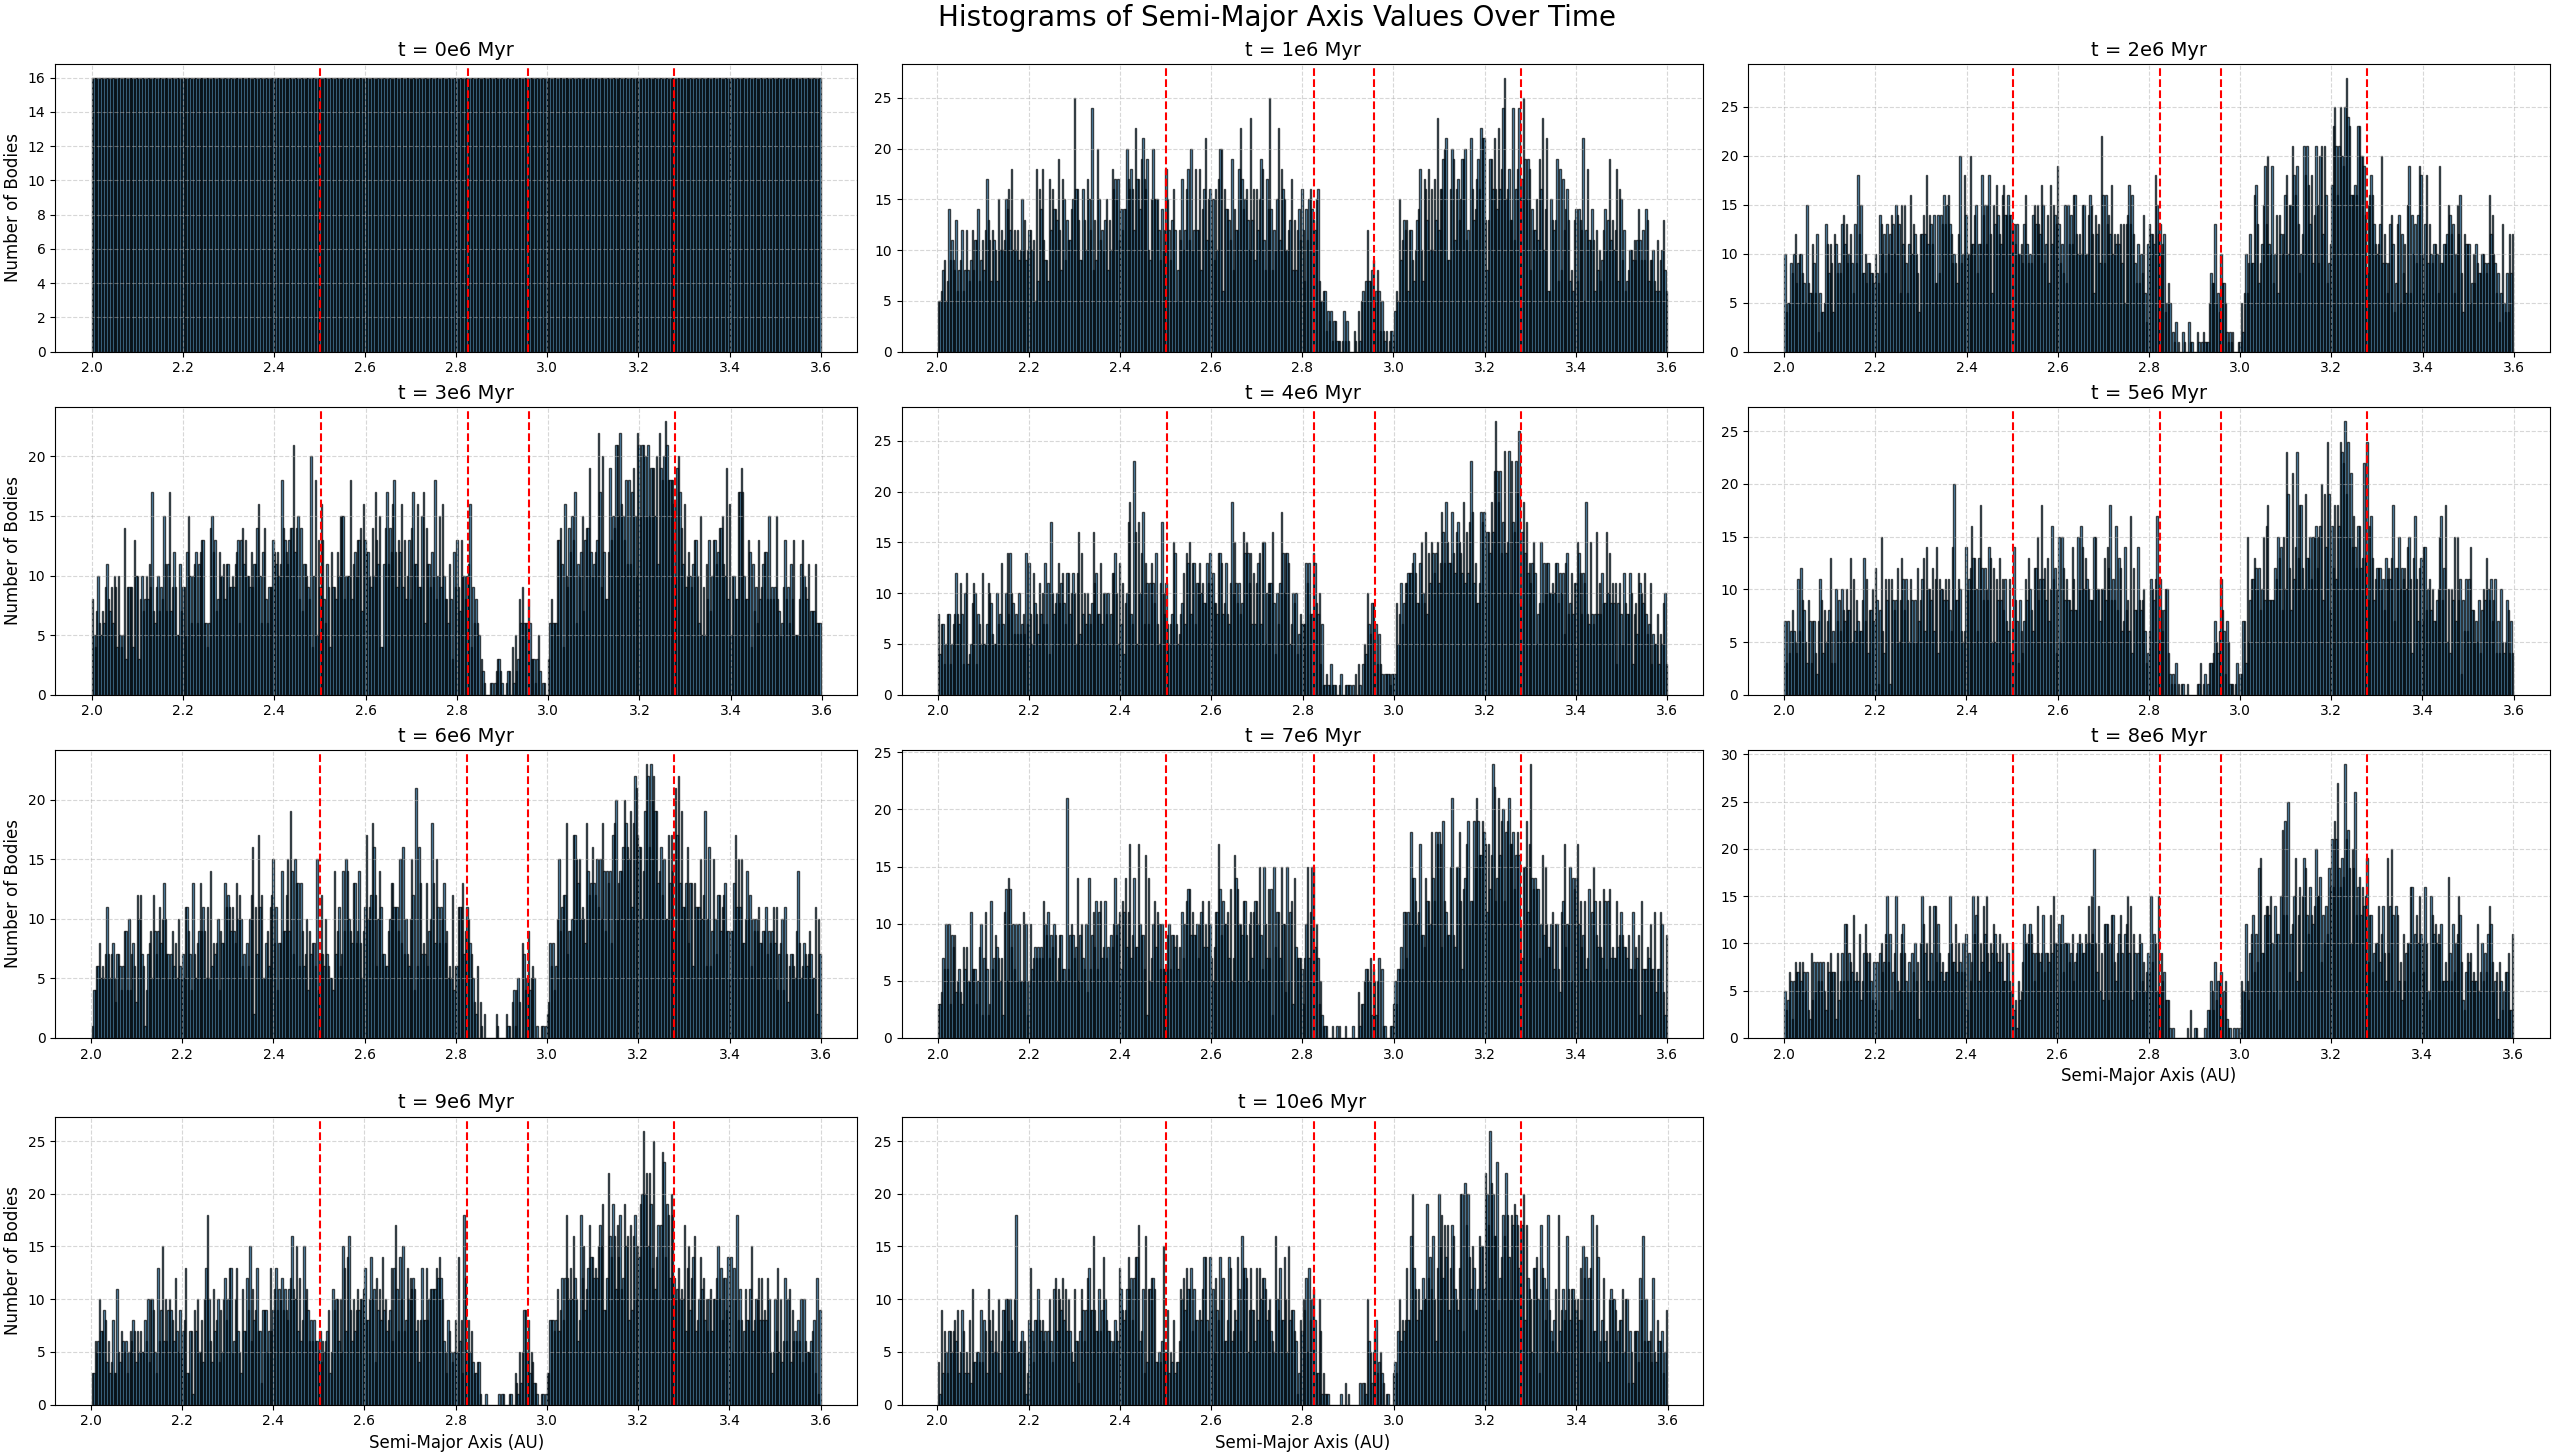
\includegraphics[width=\linewidth]{kirkwood/hist_kirkwood.png}
  \caption{Histograms of the number of asteroids at various distances every $10^5$ years. Red vertical lines correspond to actual Kirkwood gaps at 2.50, 2.82, 2.95, 3.27 AU.}
  \label{fig:kirkwood_histogram}
\end{figure}

Fig. \ref{fig:kirkwood_histogram} shows the histograms of the number of asteroids at various distances every $10^5$ years.
End result does not show the exact Kirkwood gaps due to the short timespan of the simulation and simplifications in the model and integrator. However, there are smaller number of asteroids near the expected respnance locations, especially near 2.82 AU and 2.95 AU.

Further, we can plot the semi-major axis and eccentricity of the test particles to see the evolution of the system:

\begin{figure}[ht]
  \centering
  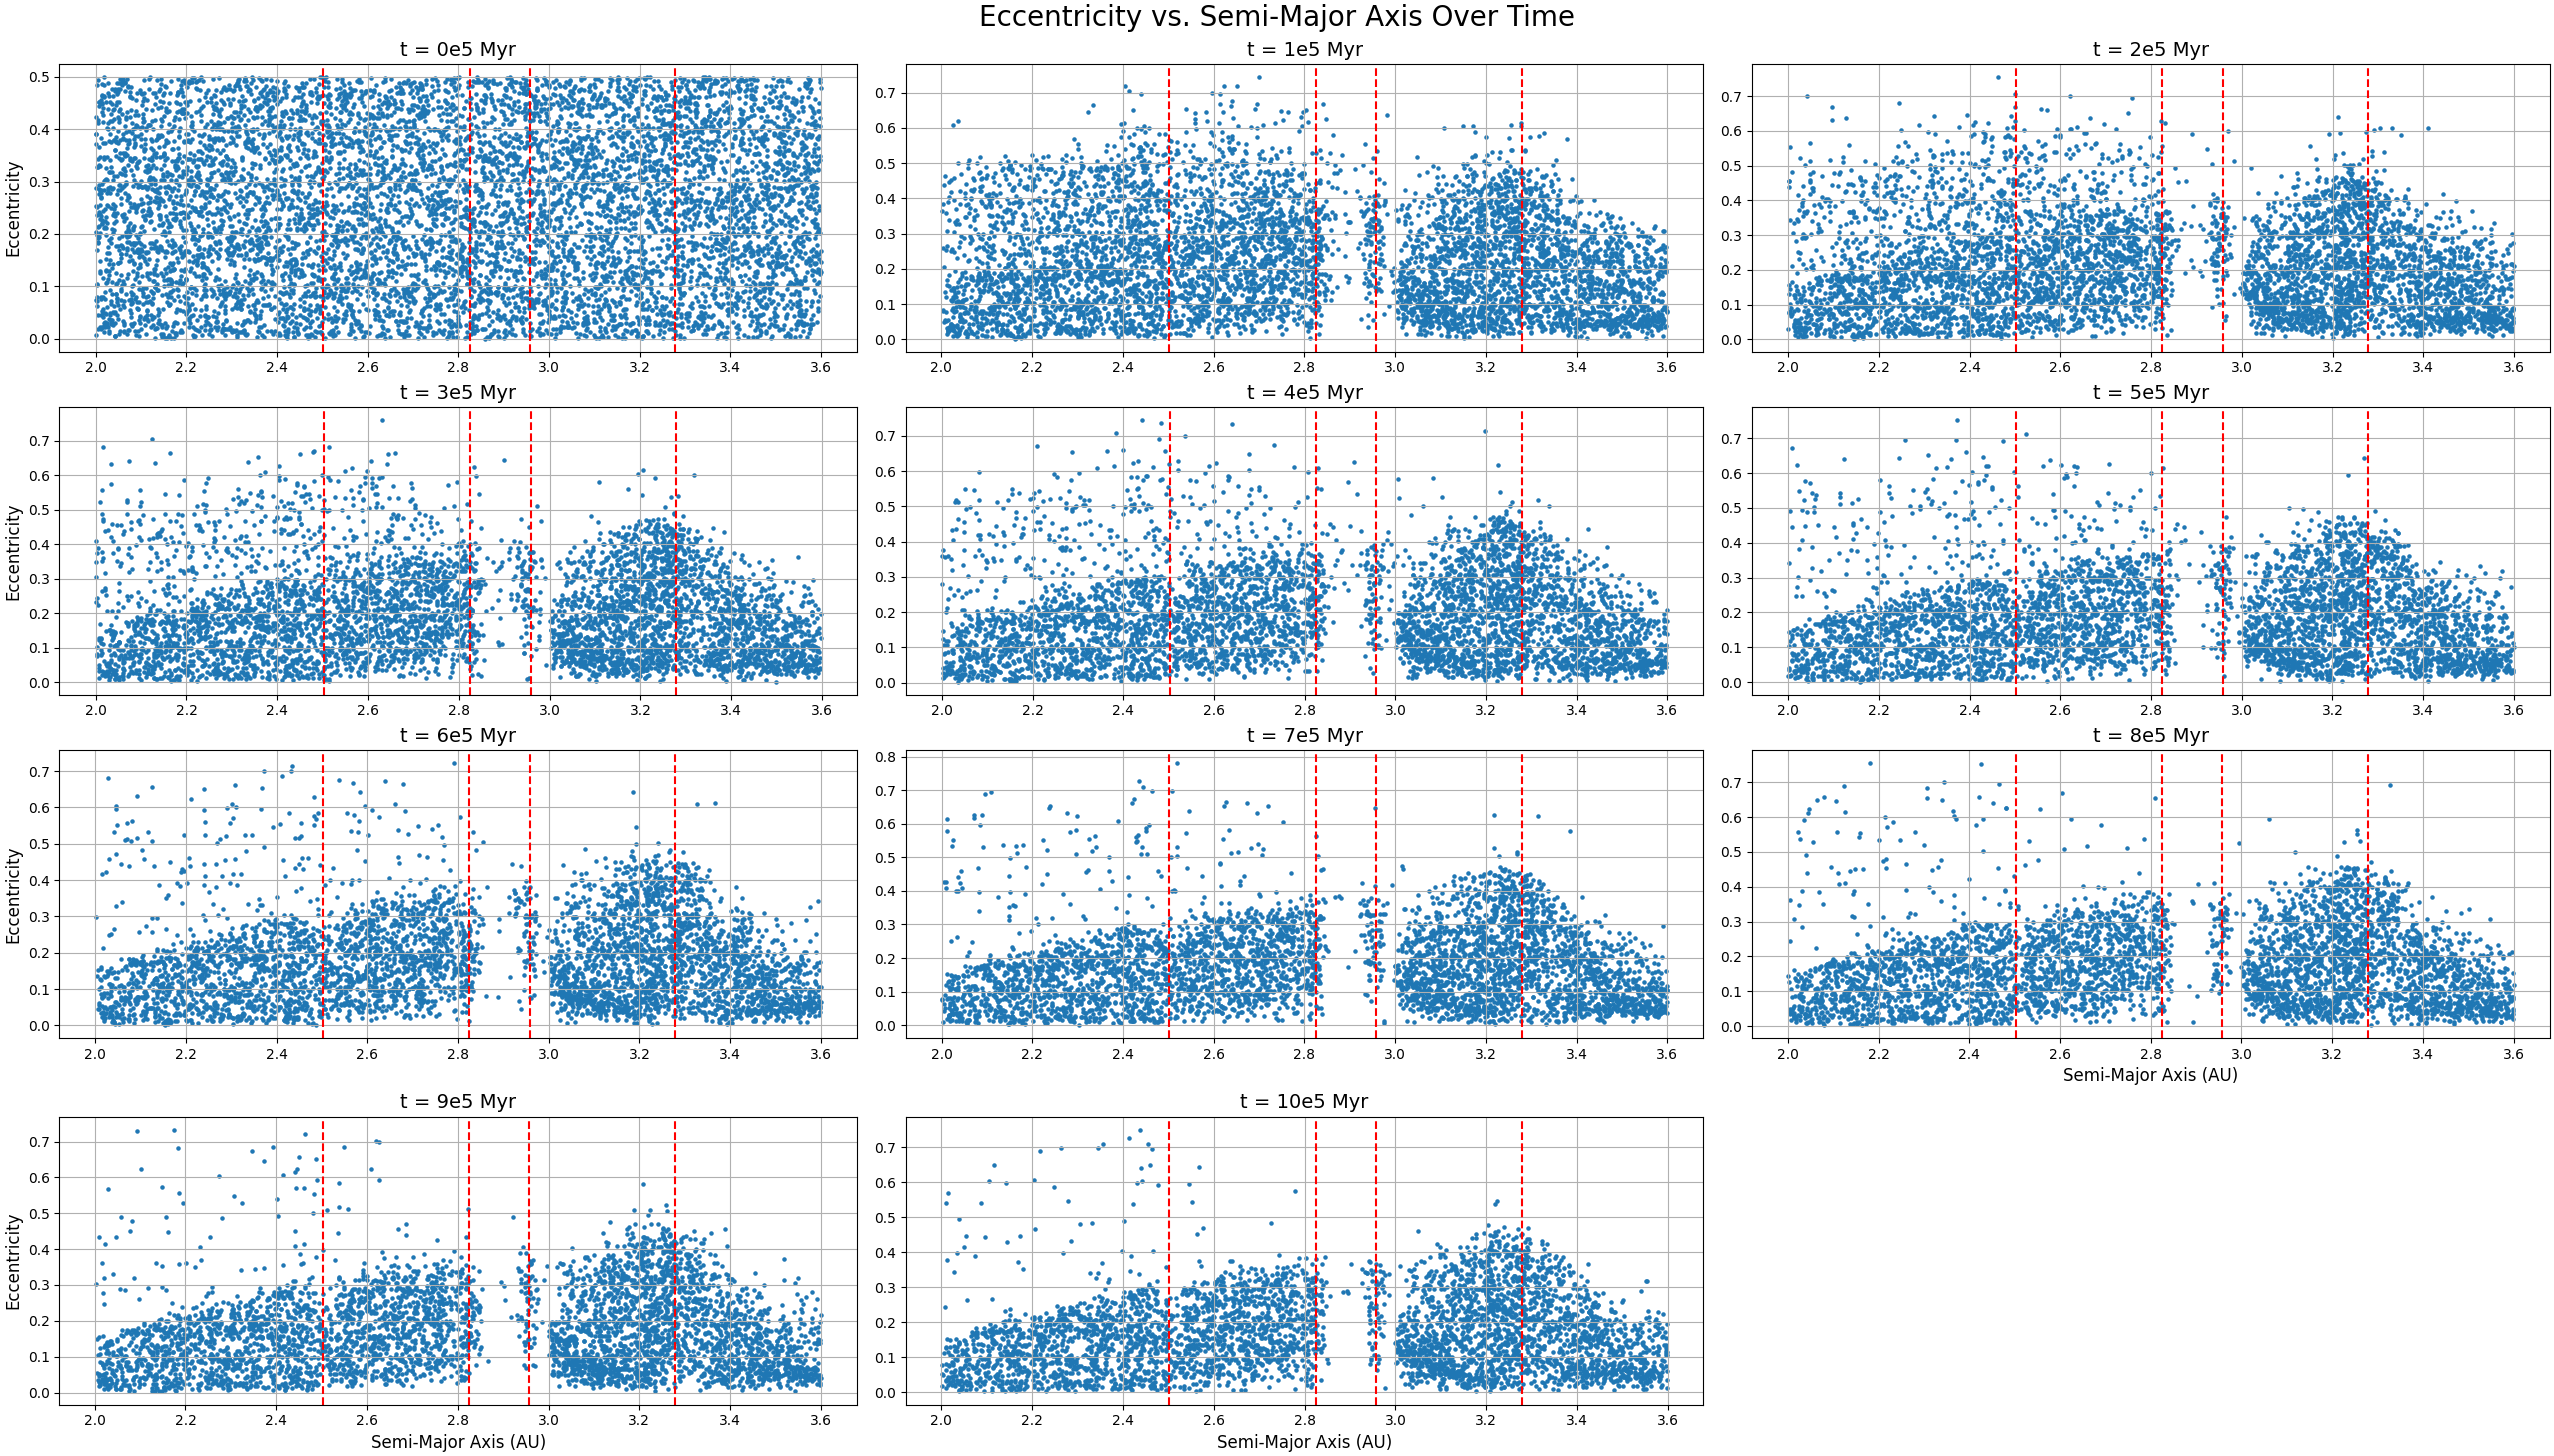
\includegraphics[width=\linewidth]{kirkwood/a_e_kirkwood.png}
  \caption{Eccentricity vs Semi-Major Axis of asteroids over time. The gaps and smaller eccentricity at smaller semi-major axis can be seen.}
  \label{fig:kirkwood_a_e}
\end{figure}

Fig. \ref{fig:kirkwood_a_e} shows the eccentricity vs semi-major axis of the asteroids over time. One can see gaps near 2.82 and 2.95 AU as well as decrease of the eccentricity at smaller orbits.
At smaller semi-major axis, objects with higher eccentricity more likely to interact with Mars, but at some even bigger eccentricities can keep being in the system at least for $10^6$ million years.

\subsection{Resonant Capture of a Planet}
This exercise investigates the effect of a Neptune-sized planet's \textbf{exponential migration} on the orbital evolution of an inner planet. Using the \texttt{REBOUND} package, we simulate the migration process and analyze how the system evolves in terms of \textbf{semimajor axes, eccentricities, and orbital period ratio.}
\\ Planetary migration is a key process in planetary system formation, occurring when planets exchange angular momentum with a gaseous protoplanetary disk or due to planet-planet interactions. During migration, planets can become locked into \textbf{mean-motion resonances (MMRs)}, which significantly influence their long-term orbital stability and eccentricities.

In this study, we simulate the migration of 'Neptune' using an \textbf{exponential migration model} and analyze how its movement affects the orbital evolution of an inner planet. We will try to track the evolution of \textbf{semimajor axes}, changes in \textbf{eccentricities}, and finally the \textbf{ratio of orbital periods} to detect resonance capture.

\subsubsection{Theory}

\textbf{1. Exponential Migration Model}

Planetary migration can be modeled as an exponential decay function:

\begin{equation}
    a(t) = a_{\text{final}} + (a_{\text{initial}} - a_{\text{final}}) e^{-t/\tau}
\end{equation}

where:
\begin{itemize}
    \item \( a_{\text{initial}} \) and \( a_{\text{final}} \) are the initial and final semimajor axes, respectively.
    \item \( \tau \) is the \textbf{e-folding time}, controlling the migration speed.
\end{itemize}

For our simulation, \textbf{Neptune migrates from 24 AU to 10 AU} with different values of \( \tau \) (\( 10^5 \) years and \( 10^6 \) years). 

\textbf{2. Resonant Capture and Mean-Motion Resonances}

When a migrating planet interacts with another body, their orbits may become \textbf{locked in resonance}, where the ratio of their orbital periods forms a simple fraction:

\begin{equation}
    \frac{P_{\text{outer}}}{P_{\text{inner}}} \approx \frac{p}{q}
\end{equation}

where \( p, q \) are small integers. Common resonances include:
\begin{itemize}
    \item \textbf{2:1 resonance} (outer planet completes 2 orbits for every 1 orbit of the inner planet).
    \item \textbf{3:2 resonance} (outer planet completes 3 orbits for every 2 of the inner planet).
\end{itemize}

Resonance capture can be detected by analyzing the \textbf{libration} of the resonant argument instead of free circulation.

\subsubsection{Simulation Setup and Code Explanation}

The simulation is performed using the \textbf{REBOUND} and \textbf{REBOUNDx} packages, with the following setup:

\textbf{1. System Initialization}
\\ A \texttt{rebound.Simulation()} object is created with the following celestial bodies:
\begin{itemize}
    \item \textbf{Sun:} Central mass of \( 1 M_{\odot} \).
    \item \textbf{Neptune:} Initially at 24 AU, mass \( 5.1 \times 10^{-5} M_{\odot} \), eccentricity 0.01.
    \item \textbf{Inner Planet:} Initially at 10 AU, mass \( 3 \times 10^{-6} M_{\odot} \), eccentricity 0.0.
\end{itemize}

\textbf{2. Exponential Migration Implementation}
\begin{itemize}
    \item \texttt{reboundx} is used to apply an exponential migration force.
    \item Two migration rates are tested:
    \begin{itemize}
        \item \textbf{Fast migration:} \( \tau = 10^5 \) years.
        \item \textbf{Slow migration:} \( \tau = 10^6 \) years.
    \end{itemize}
    \item The system is integrated for \textbf{1 million years}.
\end{itemize}

\textbf{3. Tracking Orbital Elements}
\\ During the simulation, the following are recorded:
\begin{itemize}
    \item \textbf{Eccentricity} evolution.
    \item \textbf{Semimajor axis} evolution for both planets.
    \item \textbf{Orbital period ratio}, calculated from:
    \begin{equation}
        \frac{P_{\text{Neptune}}}{P_{\text{Planet}}}
    \end{equation}
\end{itemize}

\subsubsection{Observational Analysis}
\textbf{1. Eccentricity Evolution}
\begin{figure}[h]
  \centering
  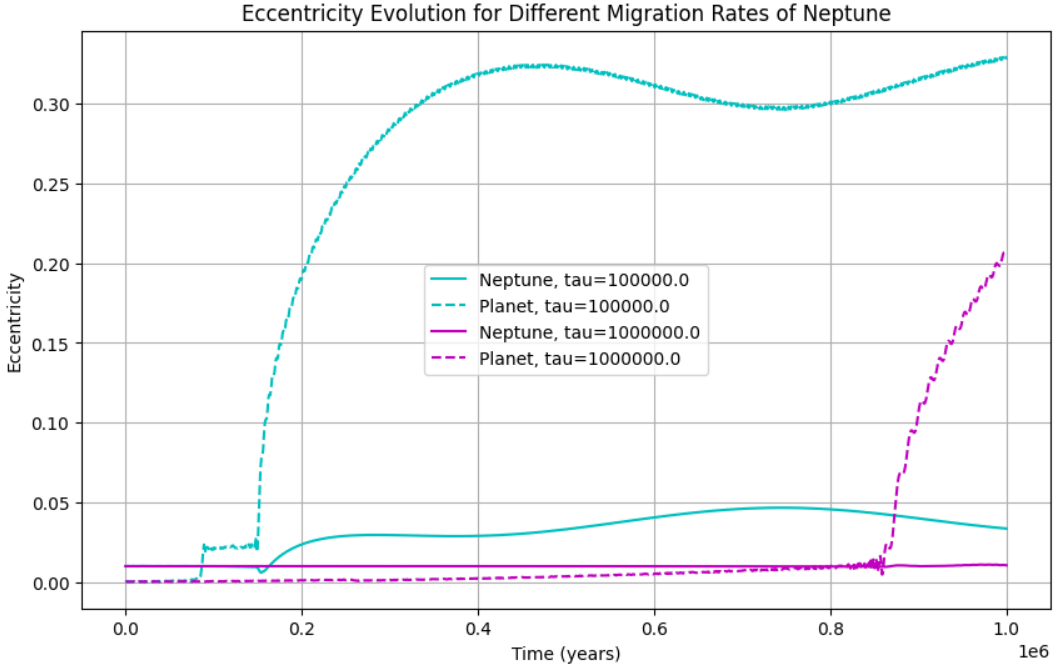
\includegraphics[width=0.8\textwidth]{ExpoMig/Eccentricity_Evo.png}
  \caption{Evolution of eccentricities of Neptune and the inner planet over time for two different migration rates.}
  \label{fig:eccentricity}
\end{figure}
\begin{itemize}
    \item For \textbf{fast migration} (\(\tau = 10^5\)), the inner planet’s eccentricity \textbf{increases significantly}, which indicates that resonance crossings are occuring more violently. 
    \\ This suggests that a faster migration of Neptune excites the inner planet's orbit strongly - indicating \textbf{resonance trapping}.
    \\ After reaching its peak, the eccentricity of the inner planet \textbf{oscillates slightly} but remains high, indicating a \textbf{dynamically excited state.}
    \item For \textbf{slow migration} (\(\tau = 10^6\)), the inner planet’s eccentricity \textbf{remains nearly zero} for most of the time, only increasing slightly toward the end.
    \\ The eccentricities of both the planets remain \textbf{relatively low} until the end of the simulation, implying that a slower, gradual migration allows for \textbf{more adiabatic evolution.} This leads to more stable, less eccentric orbits.
    \\ The slight \textbf{increase} in the inner planet's eccentricity suggests that even slow migration can eventually drive instability, though at a much later stage compared to the faster migration case.
    \item For both timescales, \textbf{Neptune's eccentricity remains small.} Since Neptune is the more massive planet, it is less affected by the resonant interactions compared to the inner planet.
    
  \end{itemize}

\textbf{2. Semimajor Axis Evolution}
\begin{figure}[h]
  \centering
  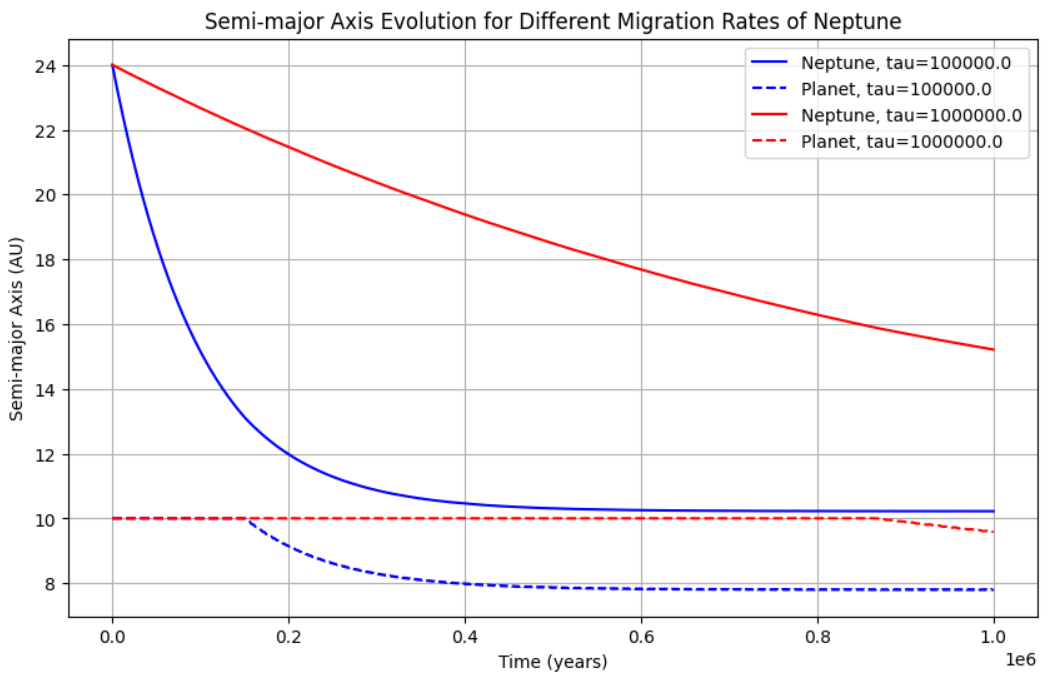
\includegraphics[width=0.8\textwidth]{ExpoMig/SemimajorAxis_Evo.png}
  \caption{Time evolution of the semimajor axes of Neptune and the inner planet for two different migration rates.}
  \label{fig:semimajor}
\end{figure}
\begin{enumerate}
    \item \textbf{Neptune's Migration}
    \begin{itemize}
      \item The blue solid line (For \(\tau = 10^5\)) shows a \textbf{rapid inward migration}, reaching a nearly constant value around 10 AU after about 300,000 years.
      \item The red solid line (For \(\tau = 10^6\)) shows a \textbf{slower inward migration}, still moving towards 10 AU but at a much more gradual rate.
    \end{itemize}
    \item \textbf{Inner Planet's Response}
    \begin{itemize}
      \item (For \(\tau = 10^5\)) (Blue dashed line):
      \\ Initially, the inner planet starts at 10 AU, meaning it is \textbf{not in resonance with Neptune at the beginning.} 
      \\ The inner planet is \textbf{strongly affected} by Neptune’s rapid movement and gets dragged inward along with it. 
      \\ Around \textbf{0.15 Myr}, the inner planet's semi-major axis \textbf{stabilizes at approximately 7.5 AU}, indicating that it has been \textbf{captured into a resonance} with Neptune.
      \item (For \(\tau = 10^6\)) (Red dashed line):
      \\ The inner planet follows a much more \textbf{gradual inward migration}, remaining around \textbf{9-10 AU} for most of the simulation.
      \\ A small final inward shift suggests that it is \textbf{slowly moving into resonance}, but in a much more controlled manner.
    \end{itemize}
    \item \textbf{Indications of Resonance Capture}
    \begin{itemize}
      \item In both cases, the inner planet \textbf{does not} continue migrating indefinitely. Instead, its migration halts once a \textbf{stable mean-motion resonance (MMR)} is reached.
      \\ Once resonance is achieved, \textbf{orbital interactions create a balance between migration forces and gravitational resonant effects}, preventing further inward drift.
      \item When Neptune migrates rapidly (For \(\tau = 10^5\)), its \textbf{gravitational perturbations are stronger}, pulling the inner planet inward more aggressively.
      \\ This process also excites the planet’s eccentricity significantly, as confirmed in the \textbf{eccentricity evolution plot} (See fig.(\ref{fig:eccentricity})).
      \\ The stronger perturbation causes capture into a \textbf{tighter resonance (3:2)}, which results in the inner planet being displaced to smaller semi-major axes (~7.5 AU).
      \item A slower migration rate (For \(\tau = 10^6\)) allows the system to gradually adjust, \textbf{making resonance capture more gentle.}
      \\ This leads to a \textbf{wider resonance (likely 2:1)}, with \textbf{less} eccentricity excitation and a \textbf{more} stable long-term configuration.
    \end{itemize}
\end{enumerate}

\textbf{3. Orbital Period Ratio Evolution}
\begin{itemize}
    \item For \textbf{fast migration (\(\tau = 10^5\))}, the period ratio quickly drops and stabilizes near 1.5. This suggests that Neptune captures the inner planet into a \textbf{3:2 mean-motion resonance (MMR)}, where Neptune completes three orbits for every two of the inner planet. The rapid drop indicates a strong interaction early in the migration, followed by a stable resonant configuration.
    \item For \textbf{slow migration (\(\tau = 10^6\))}, The period ratio gradually decreases over time instead of sharply dropping. Around 800,000 years, it stabilizes near 2.0.
    \\ This indicates a \textbf{2:1 resonance}, meaning Neptune completes two orbits for every one of the inner planet.
    \\ The \textbf{oscillations} at the end suggest some \textbf{libration around the resonance}, a typical behavior in captured resonant configurations.
\end{itemize}
\begin{figure}[h]
  \centering
  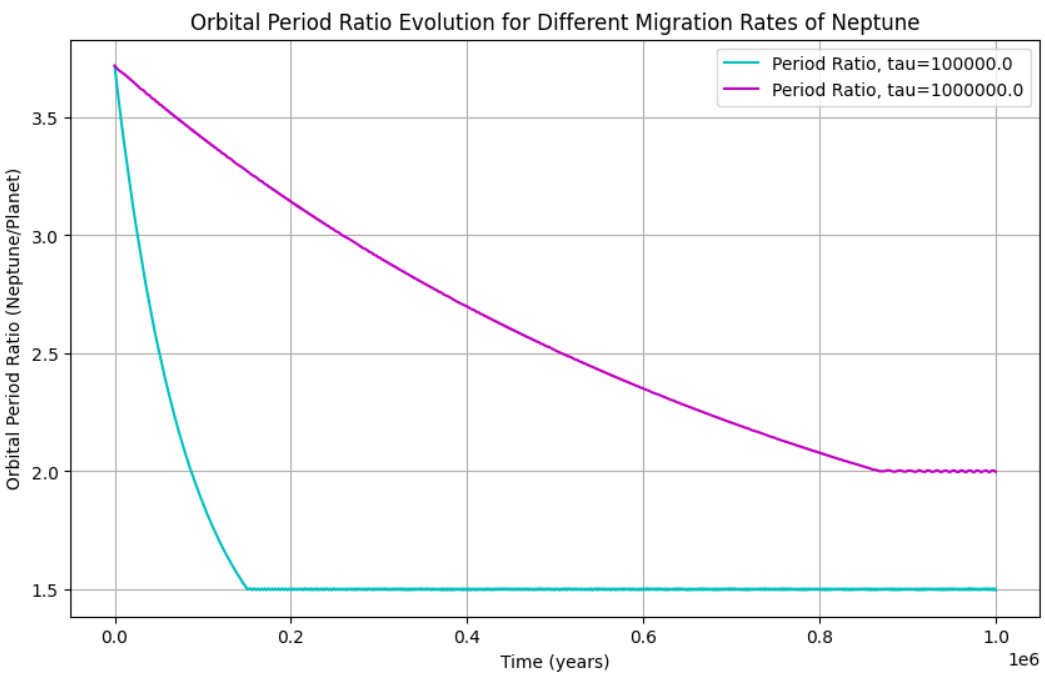
\includegraphics[width=0.8\textwidth]{ExpoMig/Period_Evo.png}
  \caption{Time evolution of the orbital period ratio of Neptune and the inner planet for two different migration rates.}
  \label{fig:period_ratio}
\end{figure}

\subsubsection{Conclusion}
\begin{itemize}
    \item \textbf{For fast migration:}
    \\ Resonant capture does occur, but the eccentricity grows significantly, possibly making the system \textbf{unstable in the long term.} 
    \\ The system reaches \textbf{a 3:2 MMR}, but the planet’s \textbf{high eccentricity} may eventually lead to further dynamical interactions.
    \item \textbf{For slow migration:}
    \\ The system reaches a \textbf{stable} resonant configuration with a \textbf{higher period ratio (a 2:1 MMR).}
    \\ The eccentricities remain low for most of the simulation, indicating \textbf{dynamical stability.}
\end{itemize}

% For each experimental part:
% \begin{enumerate}
%  \item Description of setup and procedure (1 to 3 sentences each).
%  \item Tabulated measurement results.
%  \item Analysis and graphs (including detailed calculation, giving all
% formulae and values with units used).
%  \item Discussion of result (1 to 3 sentences).
% \end{enumerate}

% \subsection{Subsection}
% You might use subsections \dots

% \subsubsection{Subsubsection}
% \dots but not more than two layers.

% And please reference all figures and tables in the text, like Figure~\ref{fig:mcp} and Table~\ref{tab:ex}.

% \begin{figure}[t]
% \centering
% 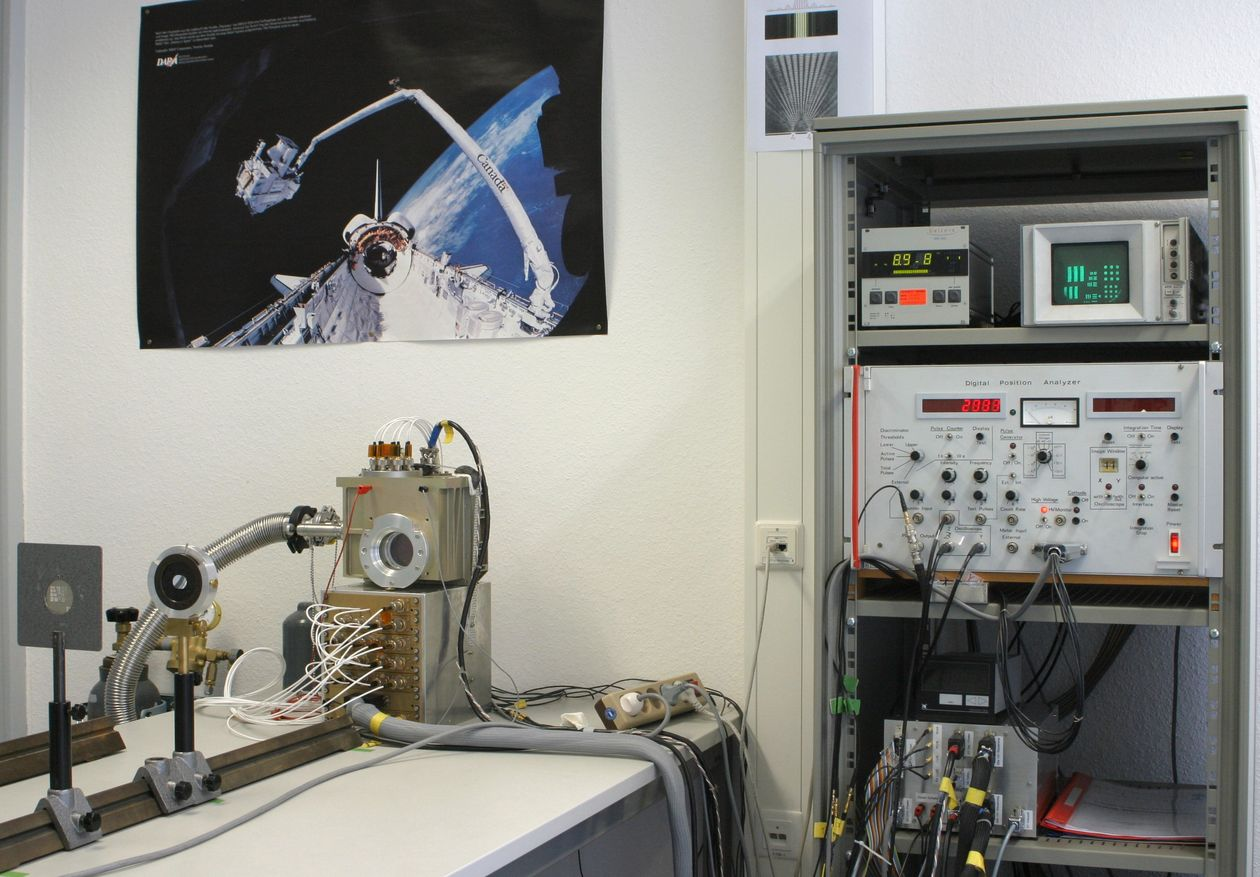
\includegraphics[width=.8\textwidth]{MCP-lab.jpg}
% \caption{All figures need a caption below. The caption should describe the figure and highlight important aspects, the rest is written in the main text. Each figure needs a reference in the text! If you are not the creator of the figure, put the appropriate citation in the caption}
% \label{fig:mcp}
% \end{figure}

% \begin{table}[t]
% 	\centering
% 	\caption{All tables need a caption above. The caption should describe the table and highlight important aspects, the rest is written in the main text. Each table needs a reference in the text! Units are given in the column headers.}
% 	\label{tab:ex}
% 	\begin{tabular}{cccc}
% 		\hline\noalign{\smallskip}
% 		Beam energy & $\Phi_\mathrm{nom}$ & $\Phi_\mathrm{app,HR}$ & $\Phi_\mathrm{app,AR}$ \\
% 		(keV) &  ($\mathrm{cm^2}$) & ($\mathrm{cm^2}$) & ($\mathrm{cm^2}$) \\
% 		\noalign{\smallskip}\hline\noalign{\smallskip}
% 		150  & $3.4 \cdot 10^{10}$ & $3.5 \cdot 10^{10}$ & $3.4 \cdot 10^{10}$ \\
% 		150  & $1.7 \cdot 10^{11}$ & $1.7 \cdot 10^{11}$ & $1.7 \cdot 10^{11}$ \\
% 		1400 & $7.5 \cdot 10^{8}$  & $9.9 \cdot 10^{8}$  & $7.4 \cdot 10^{8}$  \\
% 		\noalign{\smallskip}\hline
% 	\end{tabular}
% \end{table}

% Put also citations in the text wherever necessary and appropriate. Citations are to be used whenever external material is included, also in the text \cite{basic-contrib}, \cite{basic-online}, \cite{basic-DOI}, \cite{basic-journal}, \cite{basic-mono}.

\section{Conclusions}
  Using REBOUND we first simulated the two body problem and observed the effect of various integrators and timesteps on the accuracy of the simulation. We observed that overall IAS 15 performed the best, 
  below that WHFast and Gragg-Bulirsch-Stoer performed similarly and leapfrog was the least accurate. We also observed that the accuracy of our simulations increased with smaller timesteps.\\


  The stability of 3 body orbits with various seperations were studied. 
  \begin{enumerate}
    \item For $\Delta=0.1\Delta_c$ we observed that the planets exchanged their orbits without any collisions. 
    \item For $\Delta=0.5\Delta_c$ we observed several collisions between the planets indicating that the system was unstable.
    \item For $\Delta=1\Delta_c$, with equal masses the system was stable but unstable with unequal masses.
    \item For $\Delta=10\Delta_c$ and with equal masses, we observed that the planet closer to the star had a larger eccentricity due to tidal forces
    \item For enequal masses, the planet with smaller mass developed a larger eccentricity
  \end{enumerate}

\setcounter{secnumdepth}{0}

\printbibliography     
\appendix
\section{Appendix}
\subsection{Code}
\label{code}
  Code for 2 body and 3 body problems can be accessed from the file \texttt{NBODY.ipynb} from this folder: \url{https://unitc-my.sharepoint.com/:f:/g/personal/zxoev59_s-cloud_uni-tuebingen_de/Ehl-k6RMKhNLiHEXMrMlqkABSiXIxC3YKvn_o8Bk732B8Q?e=rOhOlq}. 
  Relevant graphs and gifs are also stored in this folder.

\end{document}

